\chapter{Graph Theory}\label{chap:graph_theory}

Informally, a graph is a bunch of dots and lines where the lines
connect some pairs of dots.  An example is shown in
Figure~\ref{fig:graph-example}.  The dots are called \emph{nodes} (or
\emph{vertices}) and the lines are called \emph{edges}.

\begin{figure}[h]
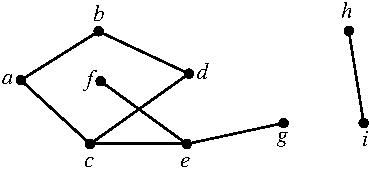
\includegraphics[height=1.5in]{graph-example}

\missinggraphic[Replace capital letters by lower]

\caption{An example of a graph with 9 nodes and 8 edges.}

\label{fig:graph-example}

\end{figure}

Graphs are ubiquitous in computer science because they provide a handy
way to represent a relationship between pairs of objects.  The objects
represent items of interest such as programs, people, cities, or web
pages, and we place an edge between a pair of nodes if they are
related in a certain way.  For example, an edge between a pair of
people might indicate that they like (or, in alternate scenarios, that
they don't like) each other.  An edge between a pair of courses might
indicate that one needs to be taken before the other.

In this chapter, we will focus our attention on simple graphs where
the relationship denoted by an edge is symmetric.  Afterward, in
Chapter~\ref{chap:digraphs}, we consider the situation where the edge
denotes a one-way relationship, that is, where one web page points to
the other.\footnote{Two Stanford students analyzed such a graph to
  become multibillionaires.  So, pay attention to graph theory, and
  who knows what might happen!}

\section{Definitions}\label{degreessec}

\subsection{Simple Graphs}

\begin{definition}\label{graphdef}
A \term{simple graph}, $G$, consists of a nonempty set,~$V$, called
the \term{vertices} (aka \emph{nodes}\footnote{We will use the terms
  vertex and node interchangeably.}) of~$G$, and a set, $E$, of
two-element subsets of $V$.  The members of $E$ are called the
\term{edges} of $G$, and we write $G = (V, E)$.
\end{definition}
The vertices correspond to the dots in Figure~\ref{fig:graph-example},
and the edges correspond to the lines.  The graph in
Figure~\ref{fig:graph-example} is expressed mathematically as $G = (V,
E)$, where:
\begin{align*}
V & =  \set{a, b, c, d, e, f, g, h, i} \\
E & =  \set{ \set{a, b}, \set{a, c}, \set{b, d}, \set{c, d},
              \set{c, e}, \set{e, f}, \set{e, g}, \set{h, i} }.
\end{align*}
It will often be helpful to use the notation $\edge{a}{b}$ for the
edge $\set{a,b}$.  Note that $\edge{a}{b}$ and $\edge{b}{a}$ are
different descriptions of the same edge, since sets are unordered.  In
this case, the graph $G = (V, E)$ has 9~nodes and 8~edges.

\begin{definition}
Two vertices in a simple graph are said to be \term{adjacent} if they are
joined by an edge, and an edge is said to be \term{incident} to the
vertices it joins.  The number of edges incident to a vertex~$v$ is called the
\term{degree} of the vertex and is denoted by $\degr{v}$;
equivalently, the degree of a vertex is
equals the number of vertices adjacent to it.
\end{definition}
For example, in the simple graph shown in
Figure~\ref{fig:fig:graph-example}, vertex~$a$ is adjacent to $b$ and
$b$ is adjacent to~$d$, and the edge $\edge{a}{c}$ is incident to
vertices $a$ and~$c$.  Vertex~$h$ has degree~1, $d$ has degree~2, and
$\degr{e} = 3$.  It is possible for a vertex to have degree~0, in
which case it is not adjacent to any other vertices.  A simple graph
does not need to have any edges at all ---in which case, the degree of
every vertex is zero and $\card{E} = 0$\footnote{The
  \emph{cardinality}, $\card{E}$, of the set~$E$ is the number of
  elements in~$E$.} ---but it does need to have at least one vertex,
that is, $\card{V} \ge 1$.

Note that simple graphs do \emph{not} have any \emph{self-loops} (\ie
an edge of the form $\{a, a\}$) since an edge is defined to be a set
of \emph{two} vertices.  In addition, there is at most one edge
between any pair of vertices in a simple graph.  In other words, a
simple graph does not contain \emph{multiedges} or \emph{multiple
  edges}.  That is because $E$ is a set.  Lastly, and most
importantly, simple graphs do not contain \emph{directed edges} (\ie
edges of the form~$(a, b)$ instead of~$\set{a, b}$).

There's no harm in relaxing these conditions, and some authors do, but
we don't need self-loops, multiple edges between the same two
vertices, or graphs with no vertices, and it's simpler not to have
them around.  We will consider graphs with directed edges (called
\emph{directed graphs} or \emph{digraphs}) at length in
Chapter~\ref{chap:digraphs}.  Since we'll only be considering simple
graphs in this chapter, we'll just call them ``graphs'' from now on.


\subsection{Some Common Graphs}

Some graphs come up so frequently that they have names.  The
\term{complete graph} on $n$ vertices, denoted $K_n$, has an edge
between every two vertices, for a total of $n(n-1)/2$ edges.  For
example, $K_5$ is shown in Figure~\ref{fig:K_5}.

\begin{figure}[h]
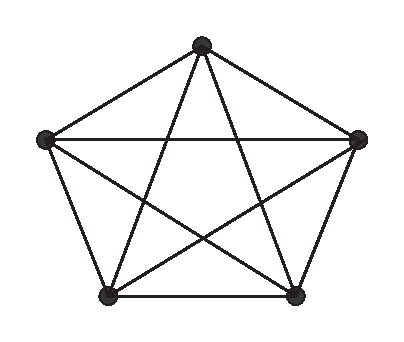
\includegraphics[height=1.5in]{complete-graph}
\caption{The complete graph on 5 nodes, $K_5$.}
\label{fig:K_5}
\end{figure}

The \term{empty graph} has no edges at all.  For example, the empty
graph with 5 nodes is shown in Figure~\ref{fig:graph_empty_5}.

\begin{figure}[h]
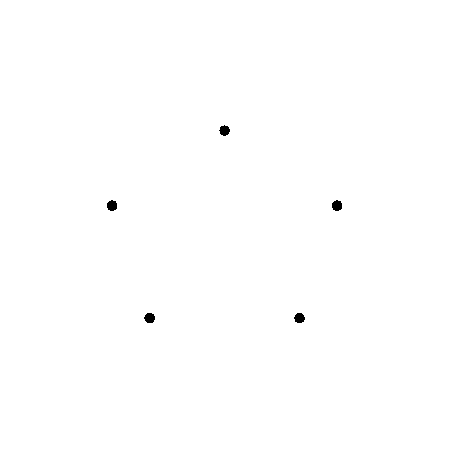
\includegraphics[height=1.5in]{empty-graph}
\caption{The empty graph with 5 nodes.}
\label{fig:graph_empty_5}
\end{figure}

The $n$-node graph containing $n - 1$ edges in sequence is known as
the \emph{line graph}~$L_n$.  More formally, $L_n = (V, E)$ where
\begin{equation*}
    V = \set{ v_1, v_2, \dots, v_n }
\end{equation*}
and
\begin{equation*}
    E = \{\, \{ v_1, v_2 \}, \{ v_2, v_3 \}, \dots, \{ v_{n-1}, v_n \} \,\}
\end{equation*}
For example, $L_5$ is displayed in Figure~\ref{fig:graph_L_5}.

\begin{figure}[h]
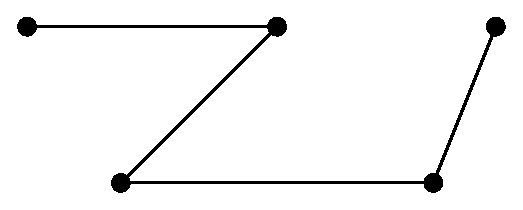
\includegraphics[height=1in]{path-graph}
\caption{The 5-node line graph~$L_5$.}
\label{fig:graph_L_5}
\end{figure}

If we add the edge $\{v_n, v_1\}$ to the line graph~$L_n$, we get the
graph $C_n$ consisting of a simple cycle.  For example, $C_5$ is
illustrated in Figure~\ref{fig:graph_C_5}.

\begin{figure}[h]
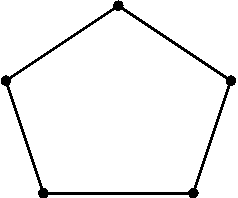
\includegraphics[height=1.5in]{cycle}
\caption{The 5-node cycle graph~$C_5$.}
\label{fig:graph_C_5}
\end{figure}

\subsection{Isomorphism}

Two graphs that look the same might actually be different in a formal
sense.  For example, the two graphs in Figure~\ref{fig:isomorphism}
are both simple cycles with 4~vertices, but one graph has vertex set
$\set{a, b, c, d}$ while the other has vertex set $\set{1, 2, 3, 4}$.
Strictly speaking, these graphs are different mathematical objects,
but this is a frustrating distinction since the graphs \emph{look the
same}!

\begin{figure}
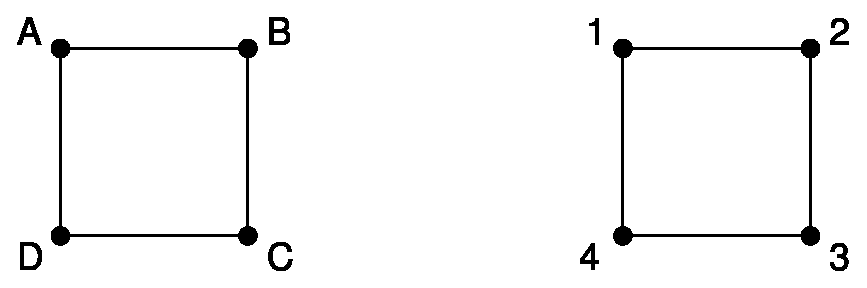
\includegraphics[height=1.5in]{isomorphism}

\missinggraphic[Add (a) and (b) sublabels; change uppercase to
  lowercase]

\caption{Two graphs that are isomorphic to~$C_4$.}
\label{fig:isomorphism}
\end{figure}

Fortunately, we can neatly capture the idea of ``looks the same''
through the notion of graph isomorphism.

\begin{definition}\label{simple-isomorphism}
If $G_1 = (V_1, E_1)$ and $G_2 = (V_2, E_2)$ are two graphs, then we
say that $G_1$ is \term{isomorphic} to $G_2$ iff there exists a
\term{bijection}\footnote{A bijection $f: V_1 \to V_2$ is a function
  that associates every node in~$V_1$ with a unique node in~$V_2$ and
  vice-versa.  We will study bijections more deeply in
  Part~\ref{part:counting}.} $f: V_1 \to V_2$ such that for every pair
of vertices $u, v \in V_1$:
\[
\edge{u}{v} \in E_1 \qiff \edge{f(u)}{f(v)} \in E_2.
\]
The function $f$ is called an \term{isomorphism} between $G_1$ and $G_2$.
\end{definition}

In other words, two graphs are isomorphic if they are the same up to a
relabeling of their vertices.
For example, here is an isomorphism between vertices in the two graphs
shown in Figure~\ref{fig:isomorphism}:
\[
\begin{array}{lll}
a \text{ corresponds to } 1 & \hspace{0.5in} & b \text{ corresponds to } 2 \\
d \text{ corresponds to } 4 & & c \text{ corresponds to } 3.
\end{array}
\]
You can check that there is an edge between two vertices in the graph
on the left if and only if there is an edge between the two
corresponding vertices in the graph on the right.

Two isomorphic graphs may be drawn very differently.  For example, we
have shown two different ways of drawing $C_5$ in
Figure~\ref{fig:isomorphism-c5}.

\begin{figure}[h]
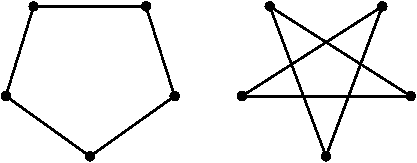
\includegraphics[height=1.5in]{isomorphism-c5}
\caption{Two ways of drawing $C_5$.}
\label{fig:isomorphism-c5}
\end{figure}

Isomorphism preserves the connection properties of a graph,
abstracting out what the vertices are called, what they are made out
of, or where they appear in a drawing of the graph.  More precisely, a
property of a graph is said to be \term{preserved under isomorphism}
if whenever $G$ has that property, every graph isomorphic to $G$ also
has that property.  For example, isomorphic graphs must have the same
number of vertices.  What's more, if $f$ is a graph isomorphism that
maps a vertex, $v$, of one graph to the vertex, $f(v)$, of an
isomorphic graph, then by definition of isomorphism, every vertex
adjacent to $v$ in the first graph will be mapped by $f$ to a vertex
adjacent to $f(v)$ in the isomorphic graph.  This means that $v$ and
$f(v)$ will have the same degree.  So if one graph has a vertex of
degree 4 and another does not, then they can't be isomorphic.  In
fact, they can't be isomorphic if the number of degree 4 vertices in
each of the graphs is not the same.

Looking for preserved properties can make it easy to determine that
two graphs are not isomorphic, or to actually find an isomorphism
between them if there is one.  In practice, it's frequently easy to
decide whether two graphs are isomorphic.  However, no one has yet
found a
\emph{general} procedure for determining whether two graphs are isomorphic
that is \emph{guaranteed} to run in polynomial
time\footnote{\emph{I.e.}, in an amount of time that is upper-bounded
  by $\card{V}^c$ where $c$ is a fixed number independent of~$\card{V}$.}
in~$\card{V}$.

Having such a procedure would be useful.  For example, it would make
it easy to search for a particular molecule in a database given the
molecular bonds.  On the other hand, knowing there is no such
efficient procedure would also be valuable: secure protocols for
encryption and remote authentication can be built on the hypothesis
that graph isomorphism is computationally exhausting.

\subsection{Subgraphs}

\begin{definition}\label{def:subgraph}
A graph $G_1 = (V_1, E_1)$ is said to be a \emph{subgraph} of a graph
$G_2 = (V_2, E_2)$ if
$V_1 \subseteq V_2$ and $E_1 \subseteq E_2$.
\end{definition}

For example, the empty graph on $n$ nodes is a subgraph of~$L_n$,
\ $L_n$ is a subgraph of~$C_n$, and $C_n$ is a subgraph of~$K_n$.
Also, the graph $G = (V, E)$ where
\begin{equation*}
    V = \{ g, h, i \} \quad \text{and}\quad  E = \{\, \{ h, i \} \,\}
\end{equation*}
is a subgraph of the graph in Figure~\ref{fig:graph-example}.  On the
other hand, any graph containing an edge~$\{g, h\}$ would not be a
subgraph of the graph in Figure~\ref{fig:graph-example} because the
graph in Figure~\ref{fig:graph-example} does not contain this edge.

Note that since a subgraph is itself a graph, the endpoints of any
edge in a subgraph must also be in the subgraph.  In other words if
$G' = (V', E')$ is a subgraph of some graph~$G$, and $\{ v_i, v_j \}
\in E'$, then it must be the case that $v_i \in V'$ and $v_j \in V'$.

\subsection{Weighted Graphs}

Sometimes, we will use edges to denote a connection between a pair of
nodes where the connection has a \emph{capacity} or \emph{weight}.
For example, we might be interested in the capacity of an internet
fiber between a pair of computers, the resistance of a wire between a
pair of terminals, the tension of a spring connecting a pair of
devices in a dynamical system, the tension of a bond between a pair of
atoms in a molecule, or the distance of a highway between a pair of
cities.

In such cases, it is useful to represent the system with an
\emph{edge-weighted} graph (aka a \emph{weighted graph}).  A weighted
graph is the same as a simple graph except that we associate a real
number (\ie the weight) with each edge in the graph.  Mathematically
speaking, a weighted graph consists of a graph $G = (V, E)$ and a
weight function $w: E \to \reals$.  For example,
Figure~\ref{fig:weighted_graph} shows a weighted graph where the
weight of edge $\edge{a}{b}$ is~5.

\begin{figure}

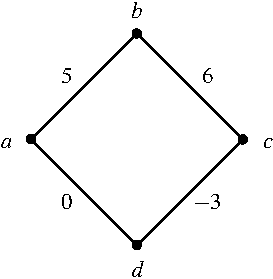
\includegraphics{Fig_5D}

\redrawn

\caption{A 4-node weighted graph where the edge~$\edge{a}{b}$ has
  weight~5.}
\label{fig:weighted_graph}
\end{figure}

\subsection{Adjacency Matrices}

There are many ways to represent a graph.  We have already seen two
ways: you can draw it, as in Figure~\ref{fig:weighted_graph} for example, or
you can represent it with sets ---as in $G = (V, E)$.  Another common
representation is with an adjacency matrix.

\begin{definition}\label{def:adjacency_matrix}

Given an $n$-node graph $G = (V, E)$ where $V = set{ v_1, v_2, \dots,
v_n }$, the \term{adjacency matrix} for~$G$ is the $n \by n$ matrix
$A_G = \set{ a_{ij} }$ where
\begin{equation*}
    a_{ij} = \begin{cases}
                1 & \text{if $\set{ v_i, v_j } \in E$} \\
                0 & \text{otherwise.}
              \end{cases}
\end{equation*}
If $G$ is a weighted graph with edge weights given by $w: E \to
\reals$, then the adjacency matrix for~$G$ is $A_G = \{ a_{ij} \}$
where
\begin{equation*}
    a_{ij} = \begin{cases}
                w(\{ v_i, v_j \}) & \text{if $\{ v_i, v_j \} \in E$} \\
                0                 & \text{otherwise.}
              \end{cases}
\end{equation*}
\end{definition}

For example, Figure~\ref{fig:adjacency_matrix} displays the adjacency
matrices for the graphs shown in Figures~\ref{fig:isomorphism}(a)
and~\ref{fig:weighted_graph} where $v_1 = a$, $v_2 = b$, $v_3 = c$,
and $v_4 = d$.

\begin{figure}[h]
\normalbaselines
\subfloat[]{%
    $
       \begin{pmatrix}
           0 & 1 & 0 & 1 \\
           1 & 0 & 1 & 0 \\
           0 & 1 & 0 & 1 \\
           1 & 0 & 1 & 0
       \end{pmatrix}
   $
}
\qquad
\subfloat[]{%
   $
       \begin{pmatrix}
           0 & 5 & 0 & 0 \\
           5 & 0 & 6 & 0 \\
           0 & 6 & 0 & -3 \\
           0 & 0 & -3 & 0
       \end{pmatrix}
   $
}

\caption{Examples of adjacency matrices.  (a)~shows the adjacency
  matrix for the graph in Figure~\ref{fig:isomorphism}(a) and
  (b)~shows the adjacency matrix for the weighted graph in
  Figure~\ref{fig:weighted_graph}.  In each case, we  set $v_1
  = a$, $v_2 = b$, $v_3 = c$, and $v_4 = d$ to construct the matrix.}
\label{fig:adjacency_matrix}
\end{figure}

%% Simple Graphs Problems %%%%%%%%%%%%%%%%%%%%%%%%%%%%%%%%%%%%%%%%%%%%%%%%%%%%%
\begin{problems}
\classproblems
\pinput{CP_Handshaking_Lemma}
\pinput{CP_isomorphic_graphs}
% S09.cp6m.1
% S09.cp6m.3
% S09.cp6m.4

\homeworkproblems
\pinput{PS_choose_isomorphic_graphs}
\pinput{PS_neighbors_under_isomorphisms}
\pinput{PS_graph_two_ends}

\examproblems
\pinput{MQ_list_isomorphisms}
\pinput{FP_bipartite_matching_sex}
\end{problems}


\section{Matching Problems}\label{sexam}

We begin our study of graph theory by considering the scenario where
the nodes in a graph represent people and the edges represent a
relationship between pairs of people such as ``likes'', ``marries'',
and so on.  Now, you may be wondering what marriage has to do with
computer science, and with good reason.  It turns out that the
techniques we will develop apply to much more general scenarios where
instead of matching men to women, we need to match packets to paths in
a network, applicants to jobs, or internet traffic to web servers.
And, as we will describe later, these techniques are widely used in
practice.

In our first example, we will show how graph theory can be used to
debunk an urban legend about sexual practices in America.  Yes, you
read correctly.  So, fasten your seat belt---who knew that math might
actually be interesting!

\subsection{Sex in America}

On average, who has more opposite-gender partners: men or women?

Sexual demographics have been the subject of many studies.  In one of the
largest, researchers from the University of Chicago interviewed a random
sample of 2500 Americans over several years to try to get an answer to this
question.  Their study, published in 1994, and entitled \emph{The Social
  Organization of Sexuality} found that, on average, men have 74\% more
opposite-gender partners than women.

Other studies have found that the disparity is even larger.  In
particular, ABC News claimed that the average man has 20 partners over his
lifetime, and the average woman has 6, for a percentage disparity of
233\%.  The ABC News study, aired on Primetime Live in 2004, purported to
be one of the most scientific ever done, with only a 2.5\% margin of
error.  It was called ``American Sex Survey: A peek between the sheets.''
The promotion for the study is even better:
\begin{quote}
``A ground breaking ABC News `Primetime Live' survey finds a range of
eye-popping sexual activities, fantasies and attitudes in this country,
confirming some conventional wisdom, exploding some myths---and venturing
where few scientific surveys have gone before.''
\end{quote}
Probably that last part about going where few scientific surveys have gone
before is pretty accurate!

Yet again, in August, 2007, the N.Y. Times reported
%% \href{The-Myth-the-Math-the-Sex.pdf}{reported}
%% \iffalse
%% \href{http://www.nytimes.com/2007/08/12/weekinreview/12kolata.html?_r=1&n=Top/Reference/Times%20Topics/People/K/Kolata,%20Gina&oref=slogin}{reported}
%% \fi
on a study by the National Center for Health Statistics of the
U.S. Government showing that men had seven partners while women had
four.

Anyway, whose numbers do you think are more accurate, the University
of Chicago, ABC News, or the National Center for Health
Statistics?---don't answer; this is a setup question like ``When did
you stop beating your wife?''  Using a little graph theory, we will
now explain why none of these findings can be anywhere near the truth.

Let's model the question of heterosexual partners in graph theoretic
terms.  To do this, we'll let $G$ be the graph whose vertices, $V$,
are all the people in America.  Then we split $V$ into two separate
subsets: $M$, which contains all the males, and $F$, which contains
all the females.\footnote{For simplicity, we'll ignore the possibility
  of someone being both, or neither, a man and a woman.}  We'll put an
edge between a male and a female iff they have been sexual partners.
A possible subgraph of this graph is illustrated in
Figure~\ref{fig:partners} with males on the left and females on the
right.

\begin{figure}[htbp]
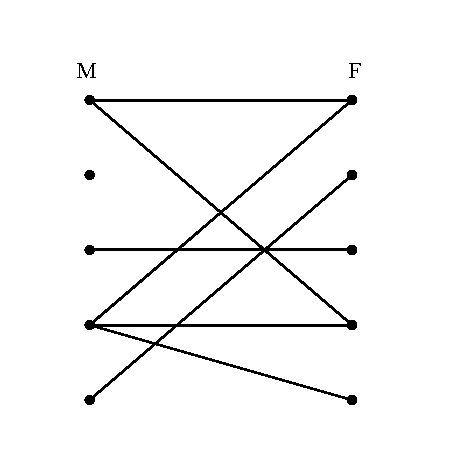
\includegraphics[height=1.75in]{sex-edges}
\caption{A possible subgraph of the sex partners graph.}
\label{fig:partners}
\end{figure}

Actually, $G$ is a pretty hard graph to figure out, let alone draw.
The graph is \emph{enormous}: the US population is about 300 million,
so $\card{V} \approx 300M$.  In the United States, approximately
50.8\% of the populatin is female and 49.2\% is male, and so $\card{M}
\approx 147.6M$, and $\card{F} \approx 152.4M$.  And we don't even
have trustworthy estimates of how many edges there are, let alone
exactly which couples are adjacent.  But it turns out that we don't
need to know any of this to debunk the sex surveys---we just need to
figure out the relationship between the average number of partners per
male and partners per female.  To do this, we note that every edge is
incident to exactly one $M$ vertex and one $F$ vertex (remember, we're
only considering male-female relationships); so the sum of the degrees
of the $M$ vertices equals the number of edges, and the sum of the
degrees of the $F$ vertices equals the number of edges.  So these sums
are equal:
%
\[
\sum_{x \in M} \degr{x} = \sum_{y \in F} \degr{y}.
\]
%
If we divide both sides of this equation by the product of the sizes
of the two sets, $\card{M} \cdot \card{F}$, we obtain
%
\begin{equation}\label{eq:average-degree}
\left(\frac{\sum_{x \in M} \degr{x}}{\card{M}}\right) \cdot \frac{1}{\card{F}} =
\left(\frac{\sum_{y \in F} \degr{y}}{\card{F}}\right) \cdot \frac{1}{\card{M}}
\end{equation}
Notice that
\begin{equation*}
    \frac{\sum_{x \in M} \degr{x}}{\card{M}}
\end{equation*}
is simply the average degree of a node in~$M$.  This is the average
number of opposite-gender partners for a male in America.  Similarly,
\begin{equation*}
    \frac{\sum_{x \in F} \degr{x}}{\card{F}}
\end{equation*}
is the average degree of a node in~$F$, which is the average number of
opposite-gender partners for a female in America.  Hence,
Equation~\ref{eq:average-degree} implies that on average, an American
male has $\card{F}/\card{M}$ times as many opposite-gender partners as the
average American female.

From the Census Bureau reports, we know that there are slightly more
females than males in America; in particular $\card{F} / \card{M}$ is
about~1.035.  So we know that on average, males have 3.5\% more
opposite-gender partners than females.  Of course, this statistic
really says nothing about
any sex's promiscuity or selectivity.  Remarkably, promiscuity is
completely irrelevant in this analysis.  That is because the ratio of
the average number of partners is completely determined by the
relative number of males and females.  Collectively, males and
females have the same number of opposite gender partners, since it
takes one of each set for every partnership, but there are fewer
males, so they have a higher ratio.  This means that the University of
Chicago, ABC, and the Federal Government studies are way off.  After a
huge effort, they gave a totally wrong answer.

There's no definite explanation for why such surveys are consistently
wrong.  One hypothesis is that males exaggerate their number of
partners---or maybe females downplay theirs---but these explanations
are speculative.  Interestingly, the principal author of the National
Center for Health Statistics study reported that she knew the results
had to be wrong, but that was the data collected, and her job was to
report it.

The same underlying issue has led to serious misinterpretations of
other survey data.  For example, a few years ago, the Boston Globe ran
a story on a survey of the study habits of students on Boston area
campuses.  Their survey showed that on average, minority students
tended to study with non-minority students more than the other way
around.  They went on at great length to explain why this ``remarkable
phenomenon'' might be true.  But it's not remarkable at all---using
our graph theory formulation, we can see that all it says is that
there are fewer minority students than non-minority students, which
is, of course what ``minority'' means.

\subsubsection{The Handshaking Lemma}

The previous argument hinged on the connection between a sum of
degrees and the number edges.  There is a simple connection between
these quantities in any graph:
\begin{lemma}[The Handshaking Lemma]\label{sumedges}
The sum of the degrees of the vertices in a graph equals twice the
number of edges.
\end{lemma}

\begin{proof}
Every edge contributes two to the sum of the degrees, one for each of
its endpoints.
\end{proof}

Lemma~\ref{sumedges} is called the \term{Handshake Lemma} because if
we total up the number of people each person at a party shakes hands
with, the total will be twice the number of handshakes that occurred.

\subsection{Bipartite Matchings}\label{bipartitesec}

\subsubsection{Bipartite Graphs}\label{bipartitesubsec}

There were two kinds of vertices in the ``Sex in America''
graph---males and females, and edges only went between the two kinds.
Graphs like this come up so frequently that they have earned a special
name---they are called \emph{bipartite graphs}.

\begin{definition}
A \term{bipartite graph} is a graph together with a partition of its
vertices into two sets, $L$ and $R$, such that every edge is incident to a
vertex in $L$ and to a vertex in $R$.
\end{definition}

So every bipartite graph looks something like the graph in
Figure~\ref{fig:partners}.

\subsubsection{The Bipartite Matching Problem}

The bipartite matching problem is related to the sex-in-America
problem that we just studied; only now the goal is to get everyone
happily married.  As you might imagine, this is not possible for a
variety of reasons, not the least of which is the fact that there are
more women in America than men.  So, it is simply not possible to
marry every woman to a man so that every man is married only once.

But what about getting a mate for every man so that every woman is
married only once?  Is it possible to do this so that each man is
paired with a woman that he likes? The answer, of course, depends on
the bipartite graph that represents who likes who, but the good news
is that it is possible to find natural properties of the who-likes-who
graph that completely determine the answer to this question.

In general, suppose that we have a set of men and an equal-sized or
larger set of women, and there is a graph with an edge between a man
and a woman if the man likes the woman.  (Note that in this scenario,
the ``likes'' relationship need not be symmetric, since for the time
being, we will only worry about finding a mate for each man that he
likes.\footnote{By the way, we do not mean to imply that marriage
  should or should not be of a heterosexual nature.  Nor do we mean to
  imply that men should get their choice instead of women.  It's just
  that with bipartite graphs, the edges only connected male nodes to
  female nodes and there are fewer men in America.  So please don't
  take offence.}  (Later, we will consider the ``likes'' relationship
from the female perspective as well.)  For example, we might obtain
the graph in Figure~\ref{fig:5J}.

\begin{problems}

\begin{editingnotes}

Move this from section \ref{bipartitesubsec} to problems.

Now we can immediately see how to color a bipartite graph using only two
colors: let all the $L$ vertices be black and all the $R$ vertices be
white.  Conversely, if a graph is 2-colorable, then it is bipartite with
$L$ being the vertices of one color and $R$ the vertices of the other
color.  In other words,
\begin{quote}
``bipartite'' is a synonym for ``\term{2-colorable}.''
\end{quote}
The following Lemma gives another useful characterization of bipartite
graphs.

\begin{theorem}\label{odd-cycle}
A graph is bipartite iff it has no odd-length cycle.
\end{theorem}
The proof of Theorem~\ref{odd-cycle} is left to
Problem~\ref{PS_no_odd_length_cycles}.
\end{editingnotes}

\end{problems}

\begin{figure}

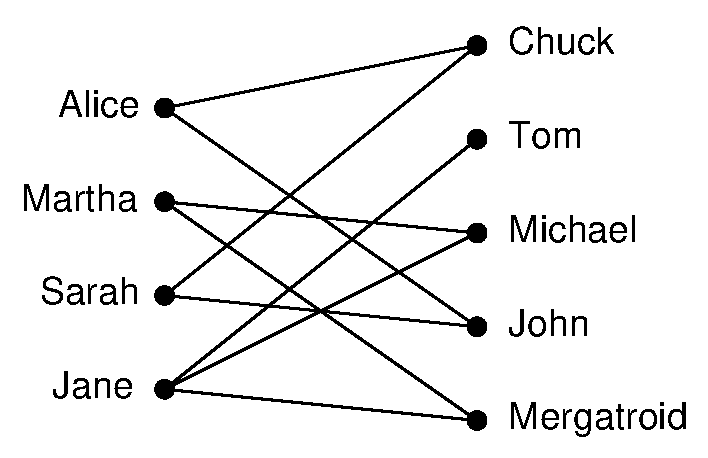
\includegraphics{hall-graph}

\redrawn

\caption{A graph where an edge between a man and woman denotes that
  the man likes the woman.}

\label{fig:5J}

\end{figure}

In this problem, a \term{matching} will mean a way of assigning every
man to a woman so that different men are assigned to different women,
and a man is always assigned to a woman that he likes.  For example,
one possible matching for the men is shown in Figure~\ref{fig:5K}.

\begin{figure}

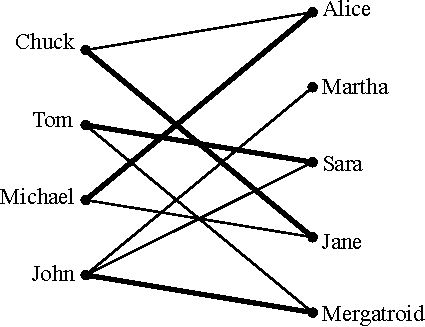
\includegraphics{hall-graph-matched}

\redrawn

\caption{One possible matching for the men is shown with bold edges.
  For example, John is matched with Jane.}

\label{fig:5K}

\end{figure}

\subsubsection{The Matching Condition}

A famous result known as \idx{Hall's Matching Theorem} gives necessary
and sufficient conditions for the existence of a matching in a
bipartite graph.  It turns out to be a remarkably useful mathematical
tool.

We'll state and prove Hall's Theorem using man-likes-woman
terminology.  Define \emph{the set of women liked by a given set of
  men} to consist of all women liked by at least one of those men.
For example, the set of women liked by Tom and John in
Figure~\ref{fig:5J} consists of Martha, Sarah, and Mergatroid.  For us
to have any chance at all of matching up the men, the following
\term{matching condition} must hold:

\medskip

\noindent\text{\emph{The Matching Condition}: every subset of men
  likes at least as large a set of women.}

\medskip

For example, we can not find a matching if some set of 4~men like only
3~women.  Hall's Theorem says that this necessary condition is
actually sufficient; if the matching condition holds, then a matching
exists.

\begin{theorem}\label{thm:matching}
A matching for a set of men~$M$ with a set of women~$W$ can be found
if and only if the matching condition holds.
\end{theorem}

\begin{proof}
First, let's suppose that a matching exists and show that the matching
condition holds.  Consider an arbitrary subset of men.  Each man likes
at least the woman he is matched with.  Therefore, every subset of men
likes at least as large a set of women.  Thus, the matching condition
holds.

Next, let's suppose that the matching condition holds and show that a
matching exists.  We use strong induction on $\card{M}$, the number of
men, on the predicate:
\begin{align*}
    P(m) ::={} & \text{for any set of $m$ men~$M$, if the matching
      condition holds} \\
             & \text{for~$M$, then there is a matching for~$M$.}
\end{align*}

\inductioncase{Base Case} ($\card{M}=1$): If $\card{M} = 1$, then the
matching condition implies that the lone man likes at least one woman,
and so a matching exists.

\inductioncase{Inductive Step:} We need to show that $P(m) \QIMPLIES
P(m + 1)$.  Suppose that $\card{M} = m + 1 \ge 2$.
\begin{description}

\item[Case 1:] Every proper subset\footnote{Recall that a subset $A$
  of~$B$ is \emph{proper} if $A \ne B$.} of men likes a \emph{strictly
  larger} set of women.  In this case, we have some latitude: we pair
  an arbitrary man with a woman he likes and send them both away.  The
  matching condition still holds for the remaining men and women since
  we have removed only one woman, so we can match the rest of the
  men by induction.

\item[Case 2:] Some proper subset of men $X \subset M$ likes an
  \emph{equal-size} set of women $Y \subset W$.  We match the men in
  $X$ with the women in $Y$ by induction and send them all away.  We
  can also match the rest of the men by induction if we show that the
  matching condition holds for the remaining men and women.  To check
  the matching condition for the remaining people, consider an
  arbitrary subset of the remaining men $X' \subseteq (M - X)$, and
  let $Y'$ be the set of remaining women that they like.  We must show
  that $\card{X'} \leq \card{Y'}$.  Originally, the combined set of
  men $X \cup X'$ liked the set of women $Y \cup Y'$.  So, by the
  matching condition, we know:
%
  \begin{equation*}
  \card{X \cup X'}  \leq  \card{Y \cup Y'}
  \end{equation*}
%
  We sent away $\card{X}$ men from the set on the left (leaving $X'$)
  and sent away an equal number of women from the set on the right
  (leaving $Y'$).  Therefore, it must be that $\card{X'} \leq
  \card{Y'}$ as claimed.
\end{description}

So in both cases, there is a matching for the men, which completes the
proof of the Inductive step.  The theorem follows by induction.
\end{proof}

The proof of Theorem~\ref{thm:matching} gives an algorithm for finding
a matching in a bipartite graph, albeit not a very efficient one.
However, efficient algorithms for finding a matching in a bipartite
graph do exist.  Thus, if a problem can be reduced to finding a
matching, the problem is essentially solved from a computational
perspective.

\subsubsection{A Formal Statement}

Let's restate Theorem~\ref{thm:matching} in abstract terms so that
you'll not always be condemned to saying, ``Now this group of men
likes at least as many women\dots''

\begin{definition}\label{def:5K}

A \term{matching} in a graph, $G$, is a set of edges such that no two
edges in the set share a vertex.  A matching is said to \emph{cover} a
set, $L$, of vertices iff each vertex in $L$ has an edge of the
matching incident to it.  A matching is said to be \emph{perfect} if
every node in the graph is incident to an edge in the matching.  In
any graph, the set $N(S)$, of \term{neighbors} of some set, $S$, of
vertices is the set of all vertices adjacent to some vertex in $S$.
That is,
\[
N(S) \eqdef \set{\,r \suchthat \edge{s}{r}\text{ is an edge for some }s \in S\,}.
\]
$S$ is called a \term{bottleneck} if
\[
\card{S} > \card{N(S)}.
\]
\end{definition}

\begin{theorem}[\idx{Hall's Theorem}]\label{thm:halls}
  Let $G$ be a bipartite graph with vertex partition $L,R$.  There is matching in $G$
  that covers $L$ iff no subset of $L$ is a bottleneck.
\end{theorem}

\subsubsection{An Easy Matching Condition}

The bipartite matching condition requires that \emph{every} subset of
men has a certain property.  In general, verifying that every subset
has some property, even if it's easy to check any particular subset
for the property, quickly becomes overwhelming because the number of
subsets of even relatively small sets is enormous---over a billion
subsets for a set of size 30.  However, there is a simple property of
vertex degrees in a bipartite graph that guarantees the existence of a
matching.  Namely, call a bipartite graph \term*{degree-constrained}
if vertex degrees on the left are at least as large as those on the
right.  More precisely,

\begin{definition}\label{degree-constrained_def}
A bipartite graph $G$ with vertex partition $L$, $R$ where $\card{L}
\le \card{R}$ is \term{degree-constrained} if $\degr{l} \geq \degr{r}$
for every $l \in L$ and $r \in R$.
\end{definition}

For example, the graph in Figure~\ref{fig:5J} is degree constrained
since every node on the left is adjacent to at least two nodes on the
right while every node on the right is incident to at most two nodes
on the left.

\begin{theorem}\label{lem:no-bottleneck}
Let $G$ be a bipartite graph with vertex partition $L$, $R$ where
$\card{L} \le \card{R}$.  If $G$ is degree-constrained, then there is
a matching that covers~$L$.
\end{theorem}

\begin{proof}
The proof is by contradiction.  Suppose that $G$ is degree constrained
but that there is no matching that covers~$L$.  By
Theorem~\ref{thm:halls}, this means that there must be a bottleneck $S
\subseteq L$.

Let $d$ be a value such that $\degr{l} \ge x \ge \degr{r}$ for every
$l \in L$ and $r \in R$.  Since every edge incident to a node in~$S$
is incident to a node in $N(S)$, we know that
\begin{equation*}
    \card{N(S)} x \ge \card{S} x
\end{equation*}
and thus that
\begin{equation*}
    \card{N(S)} \ge \card{S}.
\end{equation*}
This means that $S$ is not a bottleneck, which is a contradiction.
Hence $G$ has a matching that covers~$L$.
\end{proof}

\emph{Regular} graphs provide a large class of graphs that often arise
in practice that are degree constrained.  Hence, we can use
Theorem~\ref{lem:no-bottleneck} to prove that every regular bipartite
graph has a perfect matching.  This turns out to be a surprisingly
useful result in Computer Science

\begin{definition}\label{def:5P}
A graph is said to be \emph{regular} if every node has the same degree.
\end{definition}

\begin{theorem}\label{thm:5M}
Every regular bipartite graph has a perfect matching.
\end{theorem}

\begin{proof}
Let $G$ be a regular bipartite graph with vertex partition~$L$, $R$
where $\card{L} \leq \card{R}$.  Since regular graphs are
degree-constrained, we know by Theorem~\ref{lem:no-bottleneck} that
there must be a matching in~$G$ that covers~$L$.  Since $G$ is
regular, we also know that $\card{L} = \card{R}$ and thus the matching
must also cover~$R$.  This means that every node in~$G$ is incident to
an edge in the matching and thus $G$ has a perfect matching.
\end{proof}

\subsection{The Stable Marriage Problem}
\label{stablemarriagesec}

We next consider a version of the bipartite matching problem where
there are an equal number of men and women, and where each person has
preferences about who they would like to marry.  In fact, we assume
that each man has a complete list of all the women ranked according
to his preferences, with no ties.  Likewise, each woman has a ranked
list of all of the men.

The preferences don't have to be symmetric.  That is, Jennifer might
like Brad best, but Brad doesn't necessarily like Jennifer best.  The
goal is to marry everyone: every man must marry exactly one woman and
vice-versa---no polygamy.  Moreover, we would like to find a matching
between men and women that is \emph{stable} in the sense that there is
no pair of people that prefer each other to their spouses.

For example, suppose \emph{every} man likes Angelina best, and every
woman likes Brad best, but Brad and Angelina are married to other
people, say Jennifer and Billy Bob.  Now \emph{Brad and Angelina
  prefer each other to their spouses}, which puts their marriages at
risk: pretty soon, they're likely to start spending late nights
together working on problem sets!

This unfortunate situation is illustrated in
Figure~\ref{fig:minWtMatch2}, where the digits ``1'' and ``2'' near a
man shows which of the two women he ranks first second, respectively,
and similarly for the women.

\begin{figure}[h]
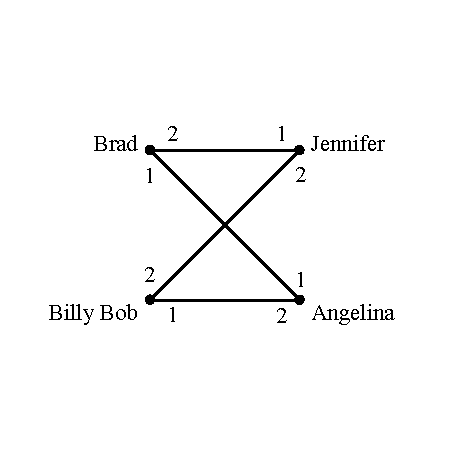
\includegraphics[height=1.2in]{minWtMatch2}

\caption{Preferences for four people.  Both men like Angelina best and
both women like Brad best.}
\label{fig:minWtMatch2}
\end{figure}

More generally, in any matching, a man and woman who are not married
to each other and who like each other better than their spouses, is
called a \emph{rogue couple}.  In the situation shown in
Figure~\ref{fig:minWtMatch2}, Brad and Angelina would be a rogue
couple.

Having a rogue couple is not a good thing, since it threatens the
stability of the marriages.  On the other hand, if there are no rogue
couples, then for any man and woman who are not married to each other,
at least one likes their spouse better than the other, and so they
won't be tempted to start an affair.

\begin{definition}
  A \term{stable matching} is a matching with no rogue couples.
\end{definition}

The question is, given everybody's preferences, how do you find a
stable set of marriages?  In the example consisting solely of the four
people in Figure~\ref{fig:minWtMatch2}, we could let Brad and Angelina
both have their first choices by marrying each other.  Now neither
Brad nor Angelina prefers anybody else to their spouse, so neither
will be in a rogue couple.  This leaves Jen not-so-happily married to
Billy Bob, but neither Jen nor Billy Bob can entice somebody else to
marry them, and so there is a stable matching.

Surprisingly, there always is a stable matching among a group of men
and women.  The surprise springs in part from considering the
apparently similar ``buddy'' matching problem.  That is, if people can
be paired off as buddies, regardless of gender, then a stable matching
\emph{may not} be possible.  For example, Figure~\ref{fig:buddy} shows
a situation with a love triangle and a fourth person who is everyone's
last choice.  In this figure Mergatroid's preferences aren't shown
because they don't even matter.  Let's see why there is no stable
matching.

\begin{figure}[htbp]
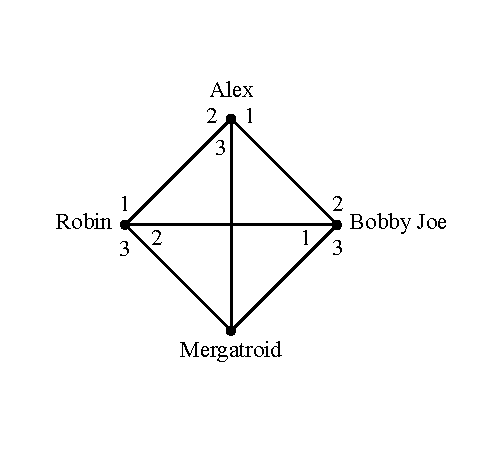
\includegraphics[height=2.3in]{loveTriangle}
\caption{Some preferences with no stable buddy matching.}
\label{fig:buddy}
\end{figure}

\begin{lemma}\label{lem:nostablematch}
There is no stable buddy matching among the four people in
Figure~\ref{fig:buddy}.
\end{lemma}

\begin{proof}
We'll prove this by contradiction.

Assume, for the purposes of contradiction, that there is a stable
matching.  Then there are two members of the love triangle that are
matched.  Since preferences in the triangle are symmetric, we may assume
in particular, that Robin and Alex are matched.  Then the other pair must
be Bobby-Joe matched with Mergatroid.

But then there is a rogue couple: Alex likes Bobby-Joe best, and Bobby-Joe
prefers Alex to his buddy Mergatroid.  That is, Alex and Bobby-Joe are a
rogue couple, contradicting the assumed stability of the matching.
\end{proof}

So getting a stable \emph{buddy} matching may not only be hard, it may
be impossible.  But when mens are only allowed to marry women, and
vice versa, then it turns out that a stable matching can always be
found.\footnote{Once again, we disclaim any political statement
  here---its just the way that the math works out.}

%%insert rest of story from gusfield book pp3--4??

\iffalse

\subsection{Failed attempts}

Let's find a stable matching in one possible situation, and hope to
translate our method to a general algorithm.  The table below shows the
preferences of each woman and man in decreasing order.

\begin{eqnarray*}
men & \quad & women \\
1 : C B E A D & \quad & A : 3 5 2 1 4 \\
2 : A B E C D & \quad & B : 5 2 1 4 3 \\
3 : D C B A E & \quad & C : 4 3 5 1 2 \\
4 : A C D B E & \quad & D : 1 2 3 4 5 \\
5 : A B D E C & \quad & E : 2 3 4 1 5
\end{eqnarray*}

How about we try a ``greedy'' strategy?\footnote{``Greedy'' is not any
moral judgment.  It refers to algorithms that work by always choosing the
next state that makes the largest immediate progress.}  We simply take
each man in turn and pack him off with his favorite among the women still
available.  This gives the following assignment.

\begin{eqnarray*}
1 \rightarrow C \\
2 \rightarrow A \\
3 \rightarrow D \\
4 \rightarrow B \\
5 \rightarrow E \\
\end{eqnarray*}

To determine whether this matching is stable, we have to check whether
there are any rogue couples.  Men 1, 2, and 3 all got their top pick
among the women; none would even think of running off.  Man~4 may be a
problem because he likes woman $A$ better than his mate, but she ranks him
dead last.  However, man~4 also likes woman $C$ better than his mate, and
she rates him above her own mate.  Therefore, man~4 and woman $C$ form a
rogue couple!  The marriages are not stable.  We could try to make ad hoc
repairs, but we're really trying to develop a general strategy.

Another approach would be to use induction.  Suppose we pair Man~1
with his favorite woman, $C$, try to show that neither of these two
will be involved in a rogue couple, and then solve the remaining
problem by induction.  Clearly Man~1 will never leave his top pick,
Woman $C$.  But the problem with this approach is that we \emph{can't}
be sure that Woman $C$ won't be in a rogue couple.  Woman $C$ might very
well dump Man~1---she might even rate him last!

This turns out to be a tricky problem.  The best approach is to use a
mating ritual that is reputed to have been popular in some mythic past.
\fi

\subsubsection{The Mating Ritual}

The procedure for finding a stable matching involves a \emph{Mating
Ritual} that takes place over several days.  The following events happen
each day:

\textbf{Morning}: Each woman stands on her balcony.  Each man stands
under the balcony of his favorite among the women on his list, and he
serenades her.  If a man has no women left on his list, he stays home
and does his math homework.

\textbf{Afternoon}: Each woman who has one or more suitors serenading
her, says to her favorite among them, ``We might get engaged.  Come
back tomorrow.''  To the other suitors, she says, ``No.  I will never
marry you!  Take a hike!''

\textbf{Evening}: Any man who is told by a woman to take a hike,
crosses that woman off his list.

\textbf{Termination condition}: When a day arrives in which every
woman has at most one suitor, the ritual ends with each woman marrying
her suitor, if she has one.

% Show example

There are a number of facts about this Mating Ritual that we would like to
prove:

\begin{itemize}
\item The Ritual eventually reaches the termination condition.
\item Everybody ends up married.
\item The resulting marriages are stable.
\end{itemize}


\subsubsection{There is a Marriage Day}

It's easy to see why the Mating Ritual has a terminal day when people
finally get married.  Every day on which the ritual hasn't terminated, at
least one man crosses a woman off his list.  (If the ritual hasn't
terminated, there must be some woman serenaded by at least two men, and at
least one of them will have to cross her off his list).  If we start with
$n$ men and $n$ women, then each of the $n$ men's lists initially has $n$
women on it, for a total of $n^2$ list entries.  Since no women ever gets
added to a list, the total number of entries on the lists decreases every
day that the Ritual continues, and so the Ritual can continue for at most
$n^2$ days.

\subsubsection{They All Live Happily Every After\dots}

We still have to prove that the Mating Ritual leaves everyone in a
stable marriage.  To do this, we note one very useful fact about the
Ritual: if a woman has a favorite suitor on some morning of the
Ritual, then that favorite suitor will still be serenading her the
next morning---because his list won't have changed.  So she is sure to
have today's favorite man among her suitors tomorrow.  That means she
will be able to choose a favorite suitor tomorrow who is at least as
desirable to her as today's favorite.  So day by day, her favorite
suitor can stay the same or get better, never worse.  This sounds like
an invariant, and it is.

\begin{definition}\label{def:P8}
Let $P$ be the predicate: For every woman, $w$, and every man, $m$, if
$w$ is crossed off $m$'s list, then $w$ has a suitor whom she prefers
over~$m$.
\end{definition}

\begin{lemma}\label{lem:5P}
$P$ is an invariant for The Mating Ritual.
\end{lemma}

\begin{proof}
By induction on the number of days.

\inductioncase{Base Case}: In the beginning (\ie at the end of day~0),
  every woman is on every list---no one has been crossed off and so
  $P$ is vacuously true.

\inductioncase{Inductive Step}: Assume $P$ is true at the end of
day~$d$ and let $w$ be a woman that has been crossed off a man $m$'s
list by the end of day~$d + 1$.

\begin{description}

\item[Case 1:]
$w$ was crossed off $m$'s list on day $d + 1$.  Then, $w$ must have a
  suitor she prefers on day~$d+1$.

\item[Case 2:]
$w$ was crossed off $m$'s list prior to day~$d+1$.  Since $P$ is true
  at the end of day~$d$, this means that $w$ has a suitor she prefers
  to~$m$ on day~$d$.  She therefore has the same suitor or someone she
  prefers better at the end of day~$d + 1$.

\end{description}
In both cases, $P$ is true at the end of day~$d + 1$ and so $P$ must
be an invariant.
\end{proof}

With Lemma~\ref{lem:5P} in hand, we can now prove:

\begin{theorem}
Everyone is married by the Mating Ritual.
\end{theorem}

\begin{proof}
By contradiction. Assume that it is the last day of the Mating Ritual
and someone does not get married.  Since there are an equal number of
men and women, and since bigamy is not allowed, this means that at
least one man (call him Bob) and at least one woman do not get
married.

Since Bob is not married, he can't be serenading anybody and so his
list must be empty.  This means that Bob has crossed every woman off
his list and so, by invariant~$P$, every woman has a suitor whom she
prefers to Bob.  Since it is the last day and every woman still has a
suitor, this means that every woman gets married.  This is a
contradiction since we already argued that at least one woman is
\emph{not} married.  Hence our assumption must be false and so
everyone must be married.
\end{proof}

\begin{theorem}
The Mating Ritual produces a stable matching.
\end{theorem}

\begin{proof}
Let Brad and Jen be any man and woman, respectively, that are
\emph{not} married to each other on the last day of the Mating Ritual.
We will prove that Brad and Jen are not a rogue couple, and thus that
all marriages on the last day are stable.  There are two cases to consider.
\begin{description}

\item[Case 1:] Jen is not on Brad's list by the end.  Then by invariant
  $P$, we know that Jen has a suitor (and hence a husband) that she
  prefers to Brad.  So she's not going to run off with Brad---Brad and
  Jen cannot be a rogue couple.

\item[Case 2:] Jen is on Brad's list.  But since Brad is not married to
  Jen, he must be choosing to serenade his wife instead of Jen, so he
  must prefer his wife.  So he's not going to run off with Jen---once
  again, Brad and Jenn are not a rogue couple.
 \qedhere

\end{description}

\end{proof}


\subsubsection{\dots Especially the Men}

Who is favored by the Mating Ritual, the men or the women?  The women
\emph{seem} to have all the power: they stand on their balconies
choosing the finest among their suitors and spurning the rest.  What's
more, we know their suitors can only change for the better as the
Ritual progresses.  Similarly, a man keeps serenading the woman he
most prefers among those on his list until he must cross her off, at
which point he serenades the next most preferred woman on his list.  So
from the man's perspective, the woman he is serenading can only change
for the worse.  Sounds like a good deal for the women.

But it's not!  The fact is that from the beginning, the men are
serenading their first choice woman, and the desirability of the woman
being serenaded decreases only enough to ensure overall stability.
The Mating Ritual actually does as well as possible for all the men
and does the worst possible job for the women.

To explain all this we need some definitions.  Let's begin by
observing that while The Mating Ritual produces one stable matching,
there may be other stable matchings among the same set of men and
women.  For example, reversing the roles of men and women will often
yield a different stable matching among them.

But some spouses might be out of the question in all possible stable
matchings.  For example, given the preferences shown in
Figure~\ref{fig:minWtMatch2}, Brad is just not in the realm of
possibility for Jennifer, since if you ever pair them, Brad and
Angelina will form a rogue couple.

\begin{definition}
Given a set of preference lists for all men and women, one person is
in another person's \emph{realm of possible spouses} if there is a
stable matching in which the two people are married.  A person's
\term{optimal spouse} is their most preferred person within their
realm of possibility.  A person's \term{pessimal spouse} is their
least preferred person in their realm of possibility.
\end{definition}

Everybody has an optimal and a pessimal spouse, since we know there is at
least one stable matching, namely the one produced by the Mating Ritual.
Now here is the shocking truth about the Mating Ritual:

\begin{theorem}\label{boyopt}
The Mating Ritual marries every man to his optimal spouse.
\end{theorem}

\begin{proof}
By contradiction.  Assume for the purpose of contradiction that some
man does not get his optimal spouse.  Then there must have been a day
when he crossed off his optimal spouse---otherwise he would still be
serenading (and would ultimately marry) her or some even more
desirable woman.

By the Well Ordering Principle, there must be a \emph{first} day when
a man (call him ``Keith'') crosses off his optimal spouse (call her
Nicole).
According to the rules of the Ritual, Keith crosses off Nicole because
Nicole has a preferred suitor (call him Tom), so
\begin{equation}
\text{Nicole prefers Tom to Keith.} \tag{$*$}
\end{equation}

Since this is the first day an optimal woman gets crossed off, we know
that Tom had not previously crossed off his optimal spouse, and so
\begin{equation}\tag{$**$}
\text{Tom ranks Nicole at least as high as his optimal spouse.}
\end{equation}
By the definition of an optimal spouse, there must be some stable set
of marriages in which Keith gets his optimal spouse, Nicole.  But then
the preferences given in~($*$) and~($**$) imply that Nicole and Tom
are a rogue couple within this supposedly stable set of marriages
(think about it).  This is a contradiction.
\end{proof}

\begin{theorem}
The Mating Ritual marries every woman to her pessimal spouse.
\end{theorem}

\begin{proof}
By contradiction.  Assume that the theorem is not true.  Hence there
must be a stable set of marriages~$\mathcal{M}$ where some woman (call
her Nicole) is married to a man (call him Tom) that she likes less
than her spouse in The Mating Ritual (call him Keith).  This means
that
\begin{equation}
\text{Nicole prefers Keith to Tom.} \tag{+}
\end{equation}

By Theorem~\ref{boyopt} and the fact that Nicole and Keith are married
in the Mating Ritual, we know that 
\begin{equation}\tag{++}
\text{Keith prefers Nicole to his spouse in~$\mathcal{M}$.}
\end{equation}
This means that Keith and Nicole form a rogue couple in~$\mathcal{M}$,
which contradicts the stability of~$\mathcal{M}$.
\end{proof}

\subsubsection{Applications}

The Mating Ritual was first announced in a paper by D. \idx{Gale} and
L.S. \idx{Shapley} in 1962, but ten years before the Gale-Shapley
paper was published, and unknown by them, a similiar algorithm was
being used to assign residents to hospitals by the National Resident
Matching Program (NRMP)\footnote{Of course, there is no serenading
  going on in the hospitals---the preferences are submitted to a
  program and the whole process is carried out by a computer.}.  The
NRMP has, since the turn of the twentieth century, assigned each
year's pool of medical school graduates to hospital residencies
(formerly called ``internships'') with hospitals and graduates playing
the roles of men and women.  (In this case, there may be multiple
women married to one man, a scenario we consider in the problem
section at the end of the chapter.).  Before the Ritual-like algorithm
was adopted, there were chronic disruptions and awkward
countermeasures taken to preserve assignments of graduates to
residencies.  The Ritual resolved these problems so successfully, that
it was used essentially without change at least through
1989.\footnote{Much more about the Stable Marriage Problem can be
  found in the very readable mathematical monograph by Dan Gusfield
  and Robert W. Irving,
  \href{http://mitpress.mit.edu/catalog/item/default.asp?ttype=2&tid=7676}{The
    Stable Marriage Problem: Structure and Algorithms}, MIT Press,
  Cambridge, Massachusetts, 1989, 240 pp.}

The internet infrastructure company, Akamai, also uses a variation of
the Mating Ritual to assign web traffic to its servers.  In the early
days, Akamai used other combinatorial optimization algorithms that got
to be too slow as the number of servers (over 65,000 in 2010) and
requests (over 800 billion per day) increased.  Akamai switched to a
Ritual-like approach since it is fast and can be run in a distributed
manner.  In this case, web requests correspond to women and web
servers correspond to men.  The web requests have preferences based on
latency and packet loss, and the web servers have preferences based on
cost of bandwidth and colocation.

Not surprisingly, the Mating Ritual is also used by at least one large
online dating agency.  Even here, there is no serenading going
on---everything is handled by computer.

\begin{problems}
\practiceproblems

\pinput{CP_mating_ritual_example}

\pinput{TP_mating_ritual_invariant}

\classproblems

\pinput{CP_mating_ritual_proof}

\pinput{CP_stable_matching_non_optimal}

\homeworkproblems

\pinput{PS_stable_matching_hospitals}

\pinput{PS_stable_matching_no_first_choice}

\pinput{PS_stable_matching_unlucky}

\begin{problem}
\begin{editingnotes}
Add problem proving that the Mating Ritual need not proceed in
morning/afternoon/evening lock step: a woman can reject nonfavorite
suitors one at a time and at any time, and a rejected man can change
the woman he serenades without waiting for the other men to change.
The proof uses the fact that single actions commute, so induction
proves that all executions are confluent---which implies all
executions end with the same man-optimal matching.  This lemma can be
cited in the planar graphs section to prove that the edges in an
embedding can be added in any order.
\end{editingnotes}
\end{problem}

\end{problems}

\section{Coloring}\label{sec:coloring}

In Section~\ref{sexam}, we used edges to indicate an affinity between
a pair of nodes.  We now consider situations where it is useful to use
edges to represent a \emph{conflict} between a pair of nodes.  For
example, consider the following exam scheduling problem.

\subsection{An Exam Scheduling Problem}

Each term, the MIT Schedules Office must assign a time slot for each
final exam.  This is not easy, because some students are taking
several classes with finals, and (even at MIT) a student can take only
one test during a particular time slot.  The Schedules Office wants to
avoid all conflicts.  Of course, you can make such a schedule by
having every exam in a different slot, but then you would need
hundreds of slots for the hundreds of courses, and the exam period
would run all year!  So, the Schedules Office would also like to keep
exam period short.

The Schedules Office's problem is easy to describe as a graph.  There
will be a vertex for each course with a final exam, and two vertices
will be adjacent exactly when some student is taking both courses.
For example, suppose we need to schedule exams for 6.041, 6.042,
6.002, 6.003 and 6.170.  The scheduling graph might appear as in
Figure~\ref{fig:5R}.

\begin{figure}

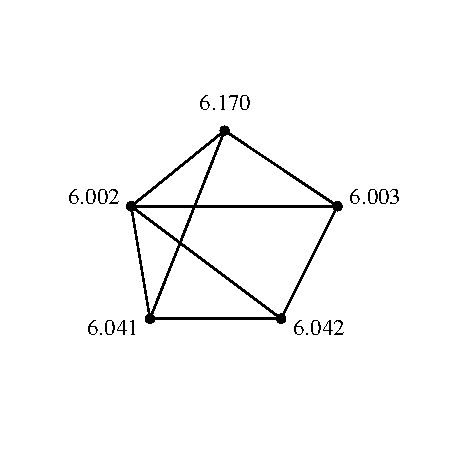
\includegraphics[height=1.5in]{finals-subject-labels}

\missinggraphic[Prefix numbers labels with ``6.'': 6.002, etc.]

\caption{A scheduling graph for five exams.  Exams connected by an
  edge cannot be given at the same time.}

\label{fig:5R}

\end{figure}

6.002 and 6.042 cannot have an exam at the same time since there are
students in both courses, so there is an edge between their nodes.  On the
other hand, 6.042 and 6.170 can have an exam at the same time if they're
taught at the same time (which they sometimes are), since no student can
be enrolled in both (that is, no student \emph{should} be enrolled in both
when they have a timing conflict).

We next identify each time slot with a color.  For example, Monday
morning is red, Monday afternoon is blue, Tuesday morning is green,
etc.  Assigning an exam to a time slot is then equivalent to coloring
the corresponding vertex.  The main constraint is that \emph{adjacent
  vertices must get different colors}---otherwise, some student has
two exams at the same time.  Furthermore, in order to keep the exam
period short, we should try to color all the vertices using as
\emph{few different colors as possible}.  As shown in Figure~\ref{fig:5S},
three colors suffice for our example.

\begin{figure}

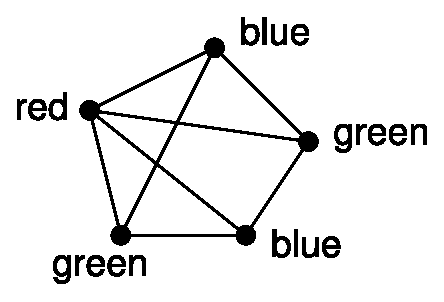
\includegraphics[height=1.5in]{finals-colored}

\caption{A 3-coloring of the exam graph from Figure~\ref{fig:5R}.}

\label{fig:5S}

\end{figure}

The coloring in Figure~\ref{fig:5S} corresponds to giving one final on
Monday morning (red), two Monday afternoon (blue), and two Tuesday
morning (green).  Can we use fewer than three colors?  No! We can't
use only two colors since there is a triangle in the graph, and three
vertices in a triangle must all have different colors.

This is an example of a \term{graph coloring problem}: given a graph
$G$, assign colors to each node such that adjacent nodes have
different colors.  A color assignment with this property is called a
\term{valid coloring} of the graph---a ``\term{coloring},'' for short.
A graph $G$ is $k$-\term{colorable} if it has a coloring that uses at
most $k$ colors.
\begin{definition}
  The minimum value of $k$ for which a graph, $G$, has a valid coloring is
  called its \term{chromatic number}, $\chi(G)$.
\end{definition}

In general, trying to figure out if you can color a graph with a fixed
number of colors can take a long time.  It's a classic example of a
problem for which no fast algorithms are known.  In fact, it is easy to
check if a coloring works, but it seems really hard to find it. (If you
figure out how, then you can get a \$1 million Clay prize.)


\subsection{Degree-Bounded Coloring}

There are some simple graph properties that give useful upper bounds
on the chromatic number.  For example, if the graph is bipartite, then
we can color it with 2 colors (one color for the nodes in the ``left''
set and a second color for the nodes in the ``right'' set).  In fact,
if the graph has any edges at all, then being bipartite is equivalent
to being 2-colorable.

Alternatively, if the graph is planar, then the famous 4-Color Theorem
says that the graph is 4-colorable.  This is a hard result to prove,
but we will come close in Section~\ref{planar_graphs_sec} where we
define planar graphs and prove that they are 5-colorable.

The chromatic number of a graph can also be shown to be small if the
vertex degrees of the graph are small.  In particular, if we have an
upper bound on the degrees of all the vertices in a graph, then we can
easily find a coloring with only one more color than the degree bound.

\begin{theorem}\label{k+1-colorable}
A graph with maximum degree at most $k$ is $(k+1)$-colorable.
\end{theorem}

The natural way to try to prove this theorem is to use induction
on~$k$.  Unfortunately, this approach leads to disaster.  It is not
that it is impossible, just that it is extremely painful and would
ruin your week if you tried it on an exam.  When you encounter such a
disaster when using induction on graphs, it is usually best to change
what you are inducting on.  In graphs, typical good choices for the
induction parameter are $n$, the number of nodes, or $e$, the number
of edges.

\begin{proof}[Proof of Theorem~\ref{k+1-colorable}]
We use induction on the number of vertices in the graph, which we
denote by $n$.  Let $P(n)$ be the proposition that an $n$-vertex graph
with maximum degree at most $k$ is $(k+1)$-colorable.

\inductioncase{Base case} ($n=1$): A 1-vertex graph has maximum degree
0 and is 1-colorable, so $P(1)$ is true.

\inductioncase{Inductive step}: Now assume that $P(n)$ is true, and
let $G$ be an $(n+1)$-vertex graph with maximum degree at most $k$.
Remove a vertex $v$ (and all edges incident to it), leaving an
$n$-vertex subgraph, $H$.  The maximum degree of $H$ is at most $k$,
and so $H$ is $(k+1)$-colorable by our assumption $P(n)$.  Now add
back vertex $v$.  We can assign $v$ a color (from the set of $k + 1$
colors) that is different from all its adjacent vertices, since there
are at most $k$ vertices adjacent to~$v$ and so at least one of the
$k+1$ colors is still available.  Therefore, $G$ is $(k+1)$-colorable.
This completes the inductive step, and the theorem follows by
induction.
\end{proof}

Sometimes $k+1$ colors is the best you can do.  For example, in the
complete graph, $K_n$, every one of its $n$ vertices is adjacent to
all the others, so all $n$ must be assigned different colors.  Of
course $n$ colors is also enough, so $\chi(K_n)=n$.  In this case,
every node has degree $k = n - 1$ and so this is an example where
Theorem~\ref{k+1-colorable} gives the best possible bound.  By a
similar argument, we can show that Theorem~\ref{k+1-colorable} gives
the best possible bound for \emph{any} graph with degree bounded by
$k$ that has $K_{k+1}$ as a subgraph.

But sometimes $k+1$ colors is far from the best that you can do.
For example, the $n$-node \emph{star graph} shown in
Figure~\ref{fig:5T} has maximum degree $n - 1$ but can be colored
using just 2 colors.

\begin{figure}

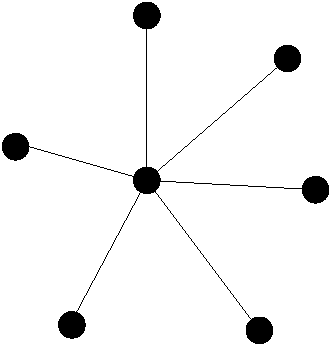
\includegraphics[height=1.5in]{star-graph}

\caption{A 7-node star graph.}

\label{fig:5T}

\end{figure}


\subsection{Why coloring?}

One reason coloring problems frequently arise in practice is because
scheduling conflicts are so common.  For example, at Akamai, a new
version of software is deployed over each of 65,000 servers every few
days.  The updates cannot be done at the same time since the servers
need to be taken down in order to deploy the software.  Also, the
servers cannot be handled one at a time, since it would take forever
to update them all (each one takes about an hour).  Moreover, certain
pairs of servers cannot be taken down at the same time since they have
common critical functions.  This problem was eventually solved by
making a 65,000-node conflict graph and coloring it with 8 colors---so
only 8 waves of install are needed!

Another example comes from the need to assign frequencies to radio
stations.  If two stations have an overlap in their broadcast area, they
can't be given the same frequency.  Frequencies are precious and
expensive, so you want to minimize the number handed out.  This amounts to
finding the minimum coloring for a graph whose vertices are the stations
and whose edges connect stations with overlapping areas.

Coloring also comes up in allocating registers for program variables.
While a variable is in use, its value needs to be saved in a register.
Registers can be reused for different variables but two variables need
different registers if they are referenced during overlapping
intervals of program execution.  So register allocation is the
coloring problem for a graph whose vertices are the variables;
vertices are adjacent if their intervals overlap, and the colors are
registers.  Once again, the goal is to minimize the number of colors
needed to color the graph.

Finally, there's the famous map coloring problem stated in
Proposition~\ref{4colorprop}.  The question is how many colors are
needed to color a map so that adjacent territories get different
colors?  This is the same as the number of colors needed to color a
graph that can be drawn in the plane without edges crossing.  A proof
that four colors are enough for \emph{planar} graphs was acclaimed
when it was discovered about thirty years ago.  Implicit in that proof
was a 4-coloring procedure that takes time proportional to the number
of vertices in the graph (countries in the map).  Surprisingly, it's
another of those million dollar prize questions to find an efficient
procedure to tell if a planar graph really \emph{needs} four colors or
if three will actually do the job.  (It's always easy to tell if an
\emph{arbitrary} graph is 2-colorable.)  In
Section~\ref{planar_graphs_sec}, we'll develop enough planar graph
theory to present an easy proof that all planar graphs are
5-colorable.

%% Connectedness %%%%%%%%%%%%%%%%%%%%%%%%%%%%%%%%%%%%%%%%%%%%%%%%%%%%%%%%%%%%%%

\section{Getting from $A$ to~$B$ in a Graph}\label{sec:connectedness}

\subsection{Paths and Walks}

\begin{definition}\label{def:undirected-path}
A \term{walk}\footnote{Some texts use the word \emph{path} for our
  definition of walk and the term \emph{simple path} for our
  definition of path.} in a graph, $G$, is a sequence of vertices
\begin{equation*}
v_0, v_1, \dots, v_k
\end{equation*}
and edges
\begin{equation*}
    \edge{v_0}{v_1}, \edge{v_1}{v_2}, \dots, \edge{v_{k - 1}}{v_k}
\end{equation*}
such that $\edge{v_i}{v_{i+1}}$ is an edge of $G$ for all $i$ where $0
\leq i < k$ .  The walk is said to \index{start of path}\emph{start}
at $v_0$, and to \index{end of walk}\emph{end} at $v_k$, and the
\index{length of walk}\emph{length} of the walk is defined to be $k$.
An edge, $\edge{u}{v}$, is \term{traversed} $n$ times by the walk if
there are $n$ different values of $i$ such that $\edge{v_i}{v_{i+1}} =
\edge{u}{v}$.  A \emph{path} is a walk where all the $v_i$'s are
different, that is, $i\neq j$ implies $v_i \neq v_j$.  For simplicity,
we will refer to paths and walks by the sequence of
vertices.\footnote{This works fine for simple graphs since the edges
  in a walk are completely determined by the sequence of vertices and
  there is no ambiguity.  For graphs with multiple edges, we would
  need to specify the edges as well as the nodes.}
\end{definition}

For example, the graph in Figure~\ref{dg} has a length~6 path $a$,
$b$, $c$, $d$, $e$, $f$,~$g$.  This is the longest path in the graph.
Of course, the graph has walks with arbitrarily large lengths, for
example, $a$, $b$, $a$, $b$, $a$, $b$,\dots.
\begin{figure}[htbp]
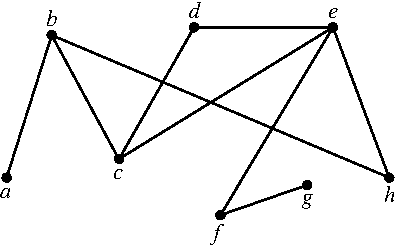
\includegraphics[height=1.75in]{distance-graph}

\missinggraphic[Change uppercase to lower]

\caption{A graph containing a path $a$, $b$, $c$, $d$, $e$, $f$,~$g$
  of length~6.}
\label{dg}
\end{figure}

The length of a walk or path is the total number of times it traverses
edges, which is \emph{one less} than its length as a sequence of
vertices.  For example, the length~6 path $a$, $b$, $c$, $d$, $e$,
$f$,~$g$ contains a sequence of 7~vertices.

\subsection{Finding a Path}

Where there's a walk, there's a path.  This is sort of obvious, but
it's easy enough to prove rigorously using the \idx{Well Ordering
  Principle}.

\begin{lemma}\label{simplepath}
If there is a walk from a vertex $u$ to a vertex~$v$ in a graph, then
there is a path from $u$ to~$v$.
\end{lemma}

\begin{proof}
Since there is a walk from $u$ to $v$, there must, by the
Well-ordering Principle, be a minimum length walk from $u$ to~$v$.  If
the minimum length is zero or one, this minimum length walk is itself
a path from $u$ to $v$.  Otherwise, there is a minimum length walk
\[
v_0, v_1, \dots, v_k
\]
from $u = v_0$ to $v = v_k$ where $k \geq 2$.  We claim this walk must
be a path.  To prove the claim, suppose to the contrary that the walk
is not a path; that is, some vertex on the walk occurs twice.  This
means that there are integers $i,j$ such that $0 \leq i < j \leq k$
with $v_i= v_j$.  Then deleting the subsequence
\[
    v_{i+1}, \dots, v_j
\]
yields a strictly shorter walk
\[
    v_0, v_1,\dots, v_i,v_{j+1},v_{j+2},\dots, v_k
\]
from $u$ to $v$, contradicting the minimality of the given walk.
\end{proof}

Actually, we proved something stronger:
\begin{corollary}\label{ss}
For any walk of length $k$ in a graph, there is a path of length
\emph{at most} $k$ with the same endpoints.  Moreover, the shortest
walk between a pair of vertices is, in fact, a path.
\end{corollary}

\subsection{Numbers of Walks}

Given a pair of nodes that are connected by a walk of length~$k$ in a
graph, there are often many walks that can be used to get from one
node to the other.  For example, there are 5 walks of length~3 that
start at~$v_1$ and end at~$v_4$ in the graph shown in
Figure~\ref{fig:5AD}.

\begin{figure}[h]

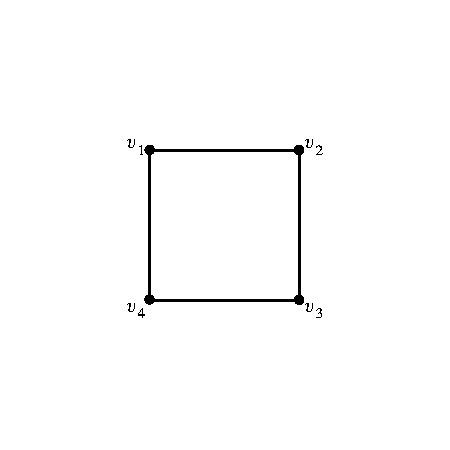
\includegraphics{Fig_5AD}

\redrawn

\caption{A graph for which there are 5 walks of length~3 from $v_1$
  to~$v_4$.  The walks are $(v_1, v_2, v_1, v_4)$, $(v_1, v_3, v_1,
  v_4)$, $(v_1, v_4, v_1, v_4)$, $(v_1, v_2, v_3, v_4)$, and $(v_1,
  v_4, v_3, v_4)$.}
\label{fig:5AD}
\end{figure}

There is a surprising relationship between the number of walks of
length~$k$ between a pair of nodes in a graph~$G$ and the $k$th power
of the adjacency matrix~$A_G$ for~$G$.  The relationship is captured
in the following theorem.

\begin{theorem}\label{thm:5AE}
Let $G = (V, E)$ be an $n$-node graph with $V = \{ v_1, v_2, \dots,
v_n \}$ and let $A_G = \{ a_{ij} \}$ denote the adjacency matrix
for~$G$.  Let $a_{ij}^{(k)}$ denote the $(i, j)$-entry of the $k$th
power of~$A_G$.  Then the number of walks of length~$k$ between $v_i$
and~$v_j$ is~$a_{ij}^{(k)}$.
\end{theorem}

In other words, we can determine the number of walks of length~$k$
between any pair of nodes simply by computing the $k$th power of the
adjacency matrix!  That's pretty amazing.

For example, the first three powers of the adjacency matrix for the
graph in Figure~\ref{fig:5AD} are:
\begin{align*}
    A &= \begin{pmatrix}
            0 & 1 & 1 & 1 \\
            1 & 0 & 1 & 0 \\
            1 & 1 & 0 & 1 \\
            1 & 0 & 1 & 0
         \end{pmatrix} & % \\[\medskipamount]
  A^2 &= \begin{pmatrix}
            3 & 1 & 2 & 1 \\
            1 & 2 & 1 & 2 \\
            2 & 1 & 3 & 1 \\
            1 & 2 & 1 & 2
         \end{pmatrix} & % \\[\medskipamount]
  A^3 &= \begin{pmatrix}
            4 & 5 & 5 & 5 \\
            5 & 2 & 5 & 2 \\
            5 & 5 & 4 & 5 \\
            5 & 2 & 5 & 2
         \end{pmatrix}
\end{align*}

Sure enough, the $(1, 4)$ coordinate of~$A^3$ is $a_{14}^{(3)} = 5$,
which is the number of length~3 walks from~$v_1$ to~$v_4$.  And
$a_{24}^{(3)} = 2$, which is the number of length~3 walks from $v_2$
to~$v_4$.  By proving the theorem, we'll discover why it is true and
thereby uncover the relationship between matrix multiplication and
numbers of walks.

\begin{proof}[Proof of Theorem~\ref{thm:5AE}]
The proof is by induction on~$k$.  We will let $P(k)$ be the predicate
that the theorem is true for~$k$.  Let $P_{ij}^{(k)}$ denote the
number of walks of length~$k$ between $v_i$ and~$v_j$.  Then $P(k)$ is
the predicate
\begin{equation}\label{eq:5AE}
    \forall i, j \in [1, n].\; P_{ij}^{(k)} = a_{ij}^{(k)}.
\end{equation}

\inductioncase{Base Case} ($k = 1$):  There are two cases to consider:
\begin{description}

\item[Case 1:]

$\{ v_i, v_j \} \in E$.  Then $P_{ij}^{(1)} = 1$ since there is
  precisely one walk of length~1 between $v_i$ and~$v_j$.  Moreover,
  $\{ v_i, v_j \} \in E$ means that $a_{ij}^{(1)} = a_{ij} = 1$.  So,
  $P_{ij}^{(1)} = a_{ij}^{(1)}$ in this case.

\item[Case 2:]

$\{ v_i, v_j \} \notin E$.  Then $P_{ij}^{(1)} = 0$ since there
  cannot be any walks of length~1 between $v_i$ and~$v_j$.  Moreover,
  $\{ v_i, v_j \} \notin E$ means that $a_{ij} = 0$.  So,
  $P_{ij}^{(1)} = a_{ij}^{(1)}$ in this case as well.

\end{description}

Hence, $P(1)$ must be true.

\inductioncase{Inductive Step}:
Assume $P(k)$ is true.  In other words, assume that
equation~\ref{eq:5AE} holds.

We can group (and thus count the number of) walks of length $k+1$
from $v_i$ to~$v_j$ according to the first edge in the walk (call it
$\{ v_i, v_t \}$).  This means that
\begin{equation}\label{eq:5AF}
    P_{ij}^{(k + 1)} = \sum^{t: \{ v_i, v_t \} \in E} P_{tj}^{(k)}
\end{equation}
where the sum is over all~$t$ such that $\{ v_i, v_t \}$ is an edge.
Using the fact that $a_{ij} = 1$ if $\{ v_i, v_t \} \in E$ and $a_{it}
= 0$ otherwise, we can rewrite Equation~\ref{eq:5AF} as follows:
\begin{equation*}
    P_{ij}^{(k + 1)} = \sum_{t = 1}^{n} a_{it} P_{tj}^{(k)}.
\end{equation*}
By the inductive hypothesis, $P_{tj}^{(k)} = a_{tj}^{(k)}$ and thus
\begin{equation*}
    P_{ij}^{(k + 1)} = \sum_{t = 1}^{n} a_{it} a_{tj}^{(k)}.
\end{equation*}
But the formula for matrix multiplication gives that
\begin{equation*}
    a_{ij}^{(k + 1)} = \sum_{t = 1}^{n} a_{it} a_{tj}^{(k)}.
\end{equation*}
and so we must have $P_{ij}^{(k+1)} = a_{ij}^{(k+1)}$ for all $i, j
\in [1, n]$.  Hence $P(k+1)$ is true and the induction is complete.
\end{proof}

\subsection{Shortest Paths}

Although the connection between the power of the adjacency matrix and
the number of walks is cool (at least if you are a mathematician), the
problem of counting walks does not come up very often in practice.
Much more important is the problem of finding the shortest path
between a pair of nodes in a graph.

There is good news and bad news to report on this front.  The good
news is that it is not very hard to find a shortest path.  The bad
news is that you can't win one of those million dollar prizes for
doing it.

In fact, there are several good algorithms known for finding a
Shortest Path between a pair of nodes.  The simplest to explain (but
not the fastest) is to compute the powers of the adjacency matrix one
by one until the value of~$a_{ij}^{(k)}$ exceeds~0.  That's because
Theorem~\ref{thm:5AE} and Corollary~\ref{ss} imply that the length of
the shortest path between $v_i$ and~$v_j$ will be the smallest value
of~$k$ for which $a_{ij}^{(k)} > 0$.

\subsubsection{Paths in Weighted Graphs}

The problem of computing shortest paths in a weighted graph frequently
arises in practice. For example, when you drive home for vacation, you
usually would like to take the shortest route.

\begin{definition}\label{def:5H}
Given a weighted graph, the length of a path in the graph is the sum
of the weights of the edges in the path.
\end{definition}

Finding shortest paths in weighted graphs is not a lot harder than
finding shortest paths in unweighted graphs.  We won't show you how to
do it here, but you will study algorithms for finding shortest paths
if you take an algorithms course.  Not surprisingly, the proof of
correctness will use induction.

\section{Connectivity}

\begin{definition}
  Two vertices in a graph are said to be \term{connected} if there
  is a path that begins at one and ends at the other.  By convention,
  every vertex is considered to be connected to itself by a path of
  length zero.
\end{definition}

\begin{definition}\label{def:connected-graph}
A graph is said to be \term{connected} when every pair of vertices are
connected.
\end{definition}

\subsection{Connected Components}

Being connected is usually a good property for a graph to have.  For
example, it could mean that it is possible to get from any node to any
other node, or that it is possible to communicate between any pair of
nodes, depending on the application.

But not all graphs are connected.  For example, the graph where nodes
represent cities and edges represent highways might be connected for
North America cities, but would surely not be connected if you also
included cities in Australia.  The same is true for communication
networks like the Internet---in order to be protected from viruses
that spread on the Internet, some government networks are completely
isolated from the Internet.

\begin{figure}[htbp]
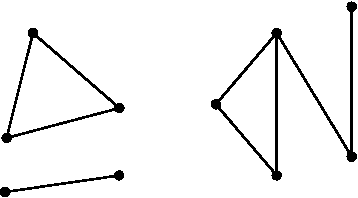
\includegraphics[height=1.5in]{connectivity-graphs}
\caption{One graph with 3 connected components.}
\label{fig:3comp}
\end{figure}

For example, the diagram in Figure~\ref{fig:3comp} looks like a
picture of three graphs, but is intended to be a picture of \emph{one}
graph.  This graph consists of three pieces (subgraphs).  Each piece
by itself is connected, but there are no paths between vertices in
different pieces.  These connected pieces of a graph are called its
\term{connected components}.

\begin{definition}\label{def:connected-component}
A \emph{connected component} is a subgraph of a graph consisting of
some vertex and every node and edge that is connected to that vertex.
\end{definition}

So a graph is connected iff it has exactly one
connected component.  The empty graph on $n$ vertices has $n$
connected components.

\subsection{$k$-Connected Graphs}

If we think of a graph as modelling cables in a telephone network, or
oil pipelines, or electrical power lines, then we not only want
connectivity, but we want connectivity that survives component
failure.  A graph is called \emph{$k$-edge connected} if it takes at
least $k$ ``edge-failures'' to disconnect it.  More precisely:

\begin{definition}
  Two vertices in a graph are $k$-\term{edge connected} if they remain
  connected in every subgraph obtained by deleting $k-1$ edges.  A graph
  with at least two vertices is $k$-edge connected\footnote{The
    corresponding definition of connectedness based on deleting vertices
    rather than edges is common in Graph Theory texts and is usually
    simply called ``$k$-connected'' rather than ``$k$-vertex connected.''}
  if every two of its vertices are $k$-edge connected.
\end{definition}

So 1-edge connected is the same as connected for both vertices and
graphs.  Another way to say that a graph is $k$-edge connected is that
every subgraph obtained from it by deleting at most $k-1$ edges is
connected.  For example, in the graph in Figure~\ref{dg}, vertices C
and~E are 3-edge connected, B and E are 2-edge connected, G and E are
1-edge connected, and no vertices are 4-edge connected.  The graph as
a whole is only 1-edge connected.  The complete graph, $K_n$, is
$(n-1)$-edge connected.

If two vertices are connected by $k$ edge-disjoint paths (that is, no
two paths traverse the same edge), then they are obviously $k$-edge
connected.  A fundamental fact, whose ingenious proof we omit,
is \idx{Menger}'s theorem which confirms that the converse is also
true: if two vertices are $k$-edge connected, then there are $k$
edge-disjoint paths connecting them.  It even takes some ingenuity to
prove this for the case $k=2$.

\subsection{The Minimum Number of Edges in a Connected Graph}

The following theorem says that a graph with few edges must have many
connected components.
\begin{theorem}\label{th:connectivity}
Every graph with $v$ vertices and $e$ edges has at least $v - e$ connected
components.
\end{theorem}
Of course for Theorem~\ref{th:connectivity} to be of any use, there must
be fewer edges than vertices.

\begin{proof}
We use induction on the number of edges, $e$.  Let $P(e)$ be the
proposition that
\begin{quote}
for every $v$, every graph with $v$ vertices and $e$ edges has at least
$v-e$ connected components.
\end{quote}

\textbf{Base case:}($e=0$).  In a graph with 0 edges and $v$ vertices,
each vertex is itself a connected component, and so there are exactly $v =
v - 0$ connected components.  So $P(e)$ holds.

\textbf{Inductive step:} Now we assume that the induction hypothesis
holds for every $e$-edge graph in order to prove that it holds for
every $(e+1)$-edge graph, where $e \geq 0$.  Consider a graph, $G$,
with $e + 1$ edges and $v$ vertices.  We want to prove that $G$ has at
least $v - (e+1)$ connected components.  To do this, remove an
arbitrary edge $\edge{a}{b}$ and call the resulting graph $G'$.  By
the induction assumption, $G'$ has at least $v - e$ connected
components.  Now add back the edge $\edge{a}{b}$ to obtain the
original graph $G$.  If $a$ and $b$ were in the same connected
component of $G'$, then $G$ has the same connected components as $G'$,
so $G$ has at least $v -e > v - (e+1)$ components.  Otherwise, if $a$
and $b$ were in different connected components of $G'$, then these two
components are merged into one component in~$G$, but all other
components remain unchanged, reducing the number of components by 1.
Therefore, $G$ has at least $(v - e) - 1 = v - (e+1)$ connected
components.  So in either case, $P(e+1)$ holds.  This completes the
Inductive step.  The theorem now follows by induction.
\end{proof}

\begin{corollary}
\label{cor:n-1}
Every connected graph with $v$ vertices has at least $v - 1$ edges.
\end{corollary}

A couple of points about the proof of Theorem~\ref{th:connectivity} are
worth noticing.  First, we used induction on the number of
edges in the graph.  This is very common in proofs involving graphs, and
so is induction on the number of vertices.  When you're presented with a
graph problem, these two approaches should be among the first you
consider.  The second point is more subtle.  Notice that in the inductive
step, we took an arbitrary $(n+1)$-edge graph, threw out an edge so that
we could apply the induction assumption, and then put the edge back.
You'll see this shrink-down, grow-back process very often in the inductive
steps of proofs related to graphs.  This might seem like needless effort;
why not start with an $n$-edge graph and add one more to get an
$(n+1)$-edge graph?  That would work fine in this case, but opens the door
to a nasty logical error called \term{buildup error}.

\subsection{Build-Up Error}

\begin{falseclm*}
If every vertex in a graph has degree at least~1, then the graph is
connected.
\end{falseclm*}

There are many counterexamples; for example, see Figure~\ref{fig:5Z}.

\begin{figure}[h]

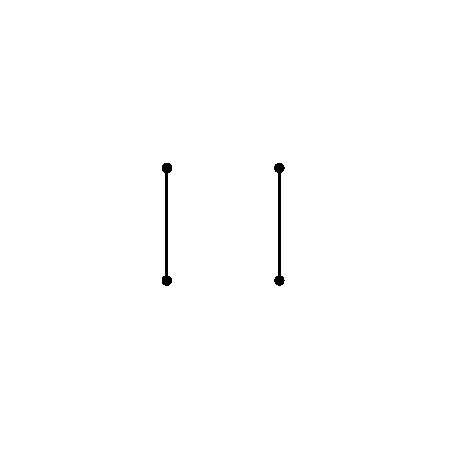
\includegraphics{Fig_5Z}

\redrawn

\caption{A counterexample graph to the False Claim.}

\label{fig:5Z}
\end{figure}

\begin{falseproof}
We use induction.  Let $P(n)$ be the proposition that if every vertex
in an $n$-vertex graph has degree at least~1, then the graph is
connected.

\inductioncase{Base case}: There is only one graph with a single
vertex and has degree~0.  Therefore, $P(1)$ is vacuously true, since
the if-part is false.

\inductioncase{Inductive step}: WE must show that $P(n)$ implies
$P(n+1)$ for all $n \ge 1$.  Consider an $n$-vertex graph in which
every vertex has degree at least~1.  By the assumption~$P(n)$, this
graph is connected; that is, there is a path between every pair of
vertices.  Now we add one more vertex~$x$ to obtain an $(n+1)$-vertex
graph as shown in Figure~\ref{fig:5Y}.

\begin{figure}[h]

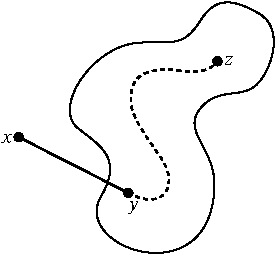
\includegraphics{Fig_5Y}

\redrawn

\caption{Adding a vertex~$x$ with degree at least~1 to a connected
  $n$-node graph.}

\label{fig:5Y}

\end{figure}

All that remains is to check that there is a path from $x$ to every
other vertex~$z$.  Since $x$ has degree at least one, there is an edge
from~$x$ to some other vertex; call it~$y$.  Thus, we can obtain a
path from~$x$ to~$z$ by adjoining the edge $\edge{x}{y}$ to the path
from~$y$ to~$z$.  This proves $P(n + 1)$.

By the principle of induction, $P(n)$ is true for all  $n \ge 1$,
which proves the theorem
\end{falseproof}

That looks fine!  Where is the bug?  It turns out that the faulty
assumption underlying this argument is that \emph{every $(n +
  1)$-vertex graph with minimum degree~1 can be obtained from an
  $n$-vertex graph with minimum degree~1 by adding 1 more vertex}.
Instead of starting by considering an arbitrary $(n + 1)$-node graph,
this proof only considered $(n + 1)$-node graphs that you can make by
starting with an $n$-node graph with minimum degree~1.

The counterexample above shows that this assumption is false; there is
no way to build the 4-vertex graph in Figure~\ref{fig:5Z} from a
3-vertex graph with minimum degree~1.  Thus the first error in the
proof is the statement ``This proves $P(n + 1)$.''

This kind of flaw is known as ``build-up error.''  Usually, build-up
error arises from a faulty assumption that every size $n + 1$ graph
with some property can be ``built up'' from a size~$n$ graph with the
same property.  (This assumption is correct for some properties, but
incorrect for others---such as the one in the argument above.)

One way to avoid an accidental build-up error is to use a ``shrink
down, grow back'' process in the inductive step: \ie start with a size
$n+1$ graph, remove a vertex (or edge), apply the inductive hypothesis
$P(n)$ to the smaller graph, and then add back the vertex (or edge)
and argue that $P(n + 1)$ holds.  Let's see what would have happened
if we'd tried to prove the claim above by this method:

\inductioncase{Revised inductive step}: We must show that $P(n)$
implies $P(n + 1)$ for all $n \ge 1$.  Consider an $(n + 1)$-vertex
graph~$G$ in which every vertex has degree at least~1.  Remove an
arbitrary vertex~$v$, leaving an $n$-vertex graph~$G'$ in which every
vertex has degree\dots\ uh oh!

The reduced graph~$G'$ might contain a vertex of degree~0, making the
inductive hypothesis $P(n)$ inapplicable!  We are stuck---and
properly so, since the claim is false!

Always use shrink-down, grow-back arguments and you'll never fall into
this trap.

%S08, cp6m, S06 cp5f

%S06 cp5f

%% Connectedness Problems %%%%%%%%%%%%%%%%%%%%%%%%%%%%%%%%%%%%%%%%%%%%%%%%%%%%
\begin{problems}
\classproblems
\pinput{CP_n_dim_hypercube}
\pinput{CP_graph_maximal_connected}
\pinput{CP_Kn_is_very_connected}
\pinput{CP_pos_deg_but_not_connected}
\homeworkproblems
\pinput{PS_Euler_circuits}

% S09.cp6m.2
% S09.cp6t.1

\homeworkproblems
\pinput{PS_tangled_and_mangled_graphs}
\pinput{PS_circuit_graph_with_crossbars}
\end{problems}

\section{Around and Around We Go}

\subsection{Cycles and Closed Walks}

\begin{definition}
A \emph{closed walk}\footnote{Some texts use the word \emph{cycle} for
  our definition of closed walk and \emph{simple cycle} for our
  definition of cycle.} in a graph~$G$ is a sequence of vertices
\begin{equation*}
    v_0, v_1, \dots, v_k
\end{equation*}
and edges
\begin{equation*}
    \edge{v_0}{v_1}, \edge{v_1}{v_2}, \dots, \edge{v_{k - 1}}{v_k}
\end{equation*}
where $v_0$ is the same node as~$v_k$ and $\edge{v_i}{v_{i + 1}}$ is
an edge of~$G$ for all~$i$ where $0 \le i < k$.  The \emph{length} of
the closed walk is~$k$.  A closed walk is said to be a \emph{cycle} if
$k \ge 3$ and $v_0$, $v_1$, \dots, $v_{k - 1}$ are all different.
\end{definition}

For example, $B$, $C$, $D$, $E$, $C$,~$B$ is a closed walk of length~5
in the graph shown in Figure~\ref{dg}. It is not a
cycle since it contains node~$C$ twice.  On the other hand, $C$, $D$,
$E$,~$C$ is a cycle of length~3 in this graph since every node appears
just once.

There are many ways to represent the same closed walk or cycle.  For
example, $B$, $C$, $D$, $E$, $C$,~$B$ is the same as $C$, $D$, $E$,
$C$, $B$,~$C$ (just starting at node~$C$ instead of node~$D$) and the
same as $B$, $C$, $E$, $D$, $C$,~$B$ (just reversing the direction).

Cycles are similar to paths, except that the last node is the first
node and the notion of first and last does not matter.  Indeed, there
are many possible vertex orders that can be used to describe cycles
and closed walks, whereas walks and paths have a prescribed beginning,
end, and ordering.

\subsection{Euler Tours}

Can you walk every hallway in the Museum of Fine Arts \emph{exactly
  once}?  If we represent hallways and intersections with edges and
vertices, then this reduces to a question about graphs.  For example,
could you visit every hallway exactly once in a museum with the
floor plan in Figure~\ref{fig:5BC}?

\begin{figure}

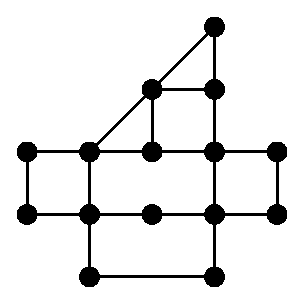
\includegraphics[height=1.5in]{euler-tour}

\caption{A possible floor plan for a museum. Can you find a walk that
  traverses every edge exactly once?}

\label{fig:5BC}

\end{figure}

The entire field of graph theory began when Euler asked whether the
seven bridges of K\"onigsberg could all be traversed exactly
once---essentially the same question we asked about the Museum of Fine
Arts.  In his honor, an \term{Euler walk} is a defined to be a walk
that traverses every edge in a graph exactly once.  Similarly, an
\term{Euler tour} is an Euler walk that starts and finishes at the
same vertex.  Graphs with Euler tours and Euler walks both have simple
characterizations.
\begin{theorem}\label{thm:euler-tour}
A connected graph has an Euler tour if and only if every vertex has
even degree.
\end{theorem}

\begin{proof}
We first show that if a graph has an Euler tour, then every vertex has
even degree.  Assume that a graph $G = (V, E)$ has an Euler tour
$v_0$, $v_1$, \dots, $v_k$ where $v_k = v_0$.  Since every edge is
traversed once in the tour, $k = \card{E}$ and the degree of a node~$u$
in~$G$ is the number of times that node appears in the sequence $v_0$,
$v_1$, \dots, $v_{k-1}$ times two.  We multiply by two since if $u =
v_i$ for some~$i$ where $0 < i < k$, then both $\edge{v_{i - 1}}{v_i}$
and $\edge{v_i}{v_{i + 1}}$ are edges incident to~$u$ in~$G$.  If $u =
v_0 = v_k$, then both $\edge{v_{k - 1}}{v_k}$ and $\edge{v_0}{v_1}$
are edges incident to~$u$ in~$G$.  Hence, the degree of every node is
even.

We next show that if the degree of every node is even in a graph $G =
(V, E)$, then there is an Euler tour.  Let
\begin{equation*}
    W ::= v_0, v_1, \dots, v_k
\end{equation*}
be the longest walk\footnote{Did you notice that we are using a
  variation of the Well Ordering Principle here when we implicitly
  assume that a longest walk exists?  This is ok since the length of a
  walk where no edge is used more than once is at most~$\card{E}$.}  in~$G$
that traverses \emph{no edge more than once}.  $W$ must traverse every
edge incident to~$v_k$; otherwise the walk could be extended and $W$
would not be the longest walk that traverses all edges at most once.
Moreover, it must be that $v_k = v_0$ and that $W$ is a closed walk,
since otherwise $v_k$ would have odd degree in~$W$ (and hence in~$G$),
which is not possible by assumption.

We conclude the argument with a proof by contradiction.  Suppose that
$W$ is not an Euler tour.  Because $G$ is a connected graph, we can
find an edge not in $W$ but incident to some vertex in $W$.  Call this
edge $\edge{u}{v_i}$.  But then we can construct a walk $W'$ that is
longer than~$W$ but that still uses no edge more than once:
\begin{equation*}
    W' ::= u, v_i, v_{i + 1}, \dots, v_k, v_1, v_2, \dots, v_i
\end{equation*}
%
This contradicts the definition of $W$, so $W$ must be an
Euler tour after all.
\end{proof}

It is not difficult to extend Theorem~\ref{thm:euler-tour} to prove that a
connected graph~$G$ has an Euler walk if and only if precisely 0 or~2
nodes in~$G$ have odd degree.  Hence, we can conclude that the graph
shown in Figure~\ref{fig:5BC} has an Euler walk but not an Euler tour
since the graph has precisely two nodes with odd degree.

Although the proof of Theorem~\ref{thm:euler-tour} does not explicitly
define a method for finding an Euler tour when one exists, it is not
hard to modify the proof to produce such a method.  The idea is to
grow a tour by continually splicing in closed walks until all the
edges are consumed.

\subsection{Hamiltonian Cycles}

Hamiltonian cycles are the unruly cousins of Euler tours.

\begin{definition}\label{def:hamiltonian-cycle}
A \emph{Hamiltonian cycle} in a graph~$G$ is a cycle that visits every
\emph{node} in~$G$ exactly once.  Similarly, a \emph{Hamiltonian} path
is a path in~$G$ that visits every node exactly once.
\end{definition}

Although Hamiltonian cycles sound similar to Euler tours---one visits
every node once while the other visits every edge once---finding a
Hamiltonian cycle can be a lot harder than finding an Euler tour.  The
same is true for Hamiltonian paths.  This is because no one has
discovered a simple characterization of all graphs with a Hamiltonian
cycle.  In fact, determining whether a graph has a Hamiltonian cycle
is the same category of problem as the SAT problem of
Section~\ref{SAT_sec}: you get a million dollars for finding an
efficient way to determine when a graph has a Hamiltonian cycle---or
proving that no procedure works efficiently on all graphs.

\subsection{The Travelling Salesperson Problem}

As if the problem of finding a Hamiltonian cycle is not hard enough,
when the graph is weighted, we often want to find a Hamiltonian cycle
that has least possible weight.  This is a very famous optimization
problem known as the Travelling Salesperson Problem.

\begin{definition}
Given a weighted graph~$G$, the \emph{weight} of a cycle in~$G$ is
defined as the sum of the weights of the edges in the cycle.
\end{definition}

For example, consider the graph shown in Figure~\ref{fig:5AL} and
suppose that you would like to visit every node once and finish at the
node where you started.  Can you find  way to do this by traversing a
cycle with weight~15?

\begin{figure}

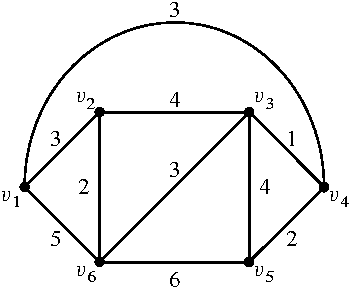
\includegraphics{Fig_5AL}

\redrawn

\caption{A weighted graph.  Can you find a cycle that visits every
  node exactly once with weight~15?}

\label{fig:5AL}
\end{figure}

Needless to say, if you can figure out a fast procedure that finds the
optimal cycle for the travelling salesperson, you can win a million
dollars.

\section{Trees}\label{trees-sec}

As we have just seen, finding good cycles in a graph can be trickier
than you might first think.  But what if a graph has no cycles at all?
Sounds pretty dull.  But graphs without cycles (called \emph{acyclic
  graphs}) are probably the most important graphs of all when it comes
to computer science.

\subsection{Definitions}

\begin{definition}\label{def:tree}
A connected acyclic graph is called a \emph{tree}.
\end{definition}

For example, Figure~\ref{fig:5H} shows an example of a 9-node tree.

\begin{figure}[h]

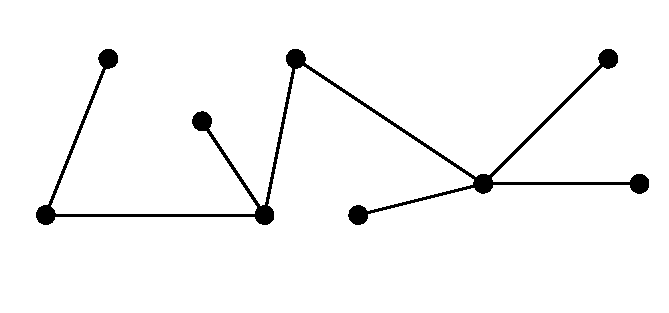
\includegraphics{tree-example}

\redrawn

\caption{A 9-node tree.}
\label{fig:5H}
\end{figure}

The graph shown in Figure~\ref{fig:5I} is not a tree since it is not
connected, but it is a forest.  That's because, of course, it consists
of a collection of trees.

\begin{definition}\label{def:forest}
If every connected component of a graph~$G$ is a tree, then $G$ is a
\emph{forest}.
\end{definition}

\begin{figure}

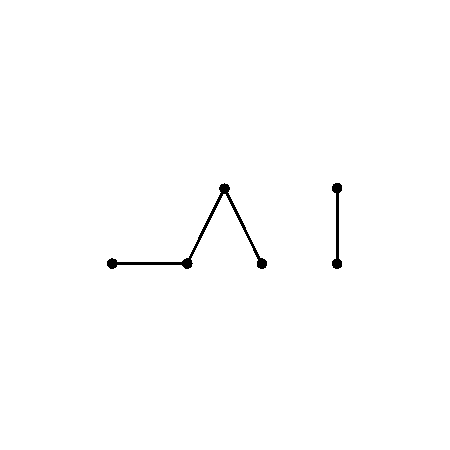
\includegraphics{Fig_5I}

\redrawn

\caption{A 6-node forest consisting of 2 component trees.  Note that
  this 6-node graph is not itself a tree since it is not connected.}
\label{fig:5I}
\end{figure}

One of the first things you will notice about trees is that they tend
to have a lot of nodes with degree one.  Such nodes are called
\emph{leaves}.

\begin{definition}
A \emph{leaf} is a node with degree~1 in a tree (or forest).
\end{definition}

For example, the tree in Figure~\ref{fig:5H} has 5 leaves and the
forest in Figure~\ref{fig:5I} has 4 leaves.

Trees are a fundamental data structure in computer science.  For
example, information is often stored in tree-like data structures and
the execution of many recursive programs can be modelled as the
traversal of a tree.  In such cases, it is often useful to draw the
tree in a levelled fashion where the node in the top level is
identified as the \emph{root}, and where every edge joins a
\emph{parent} to a \emph{child}.  For example, we have redrawn the
tree from Figure~\ref{fig:5H} in this fashion in Figure~\ref{fig:5JJ}.
In this example, node~$D$ is a child of node~$E$ and a parents of
nodes $B$ and~$C$.

\begin{figure}

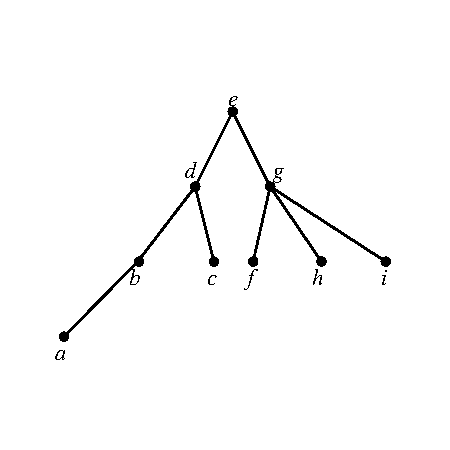
\includegraphics{Fig_5JJ}

\redrawn

\caption{The tree from Figure~\ref{fig:5H} redrawn in a leveled
  fashion, with node~$E$ as the root.}

\label{fig:5JJ}
\end{figure}

In the special case of \emph{ordered binary trees}, every node is the
parent of at most 2 children and the children are labeled as being a
left-child or a right-child.

\subsection{Properties}

Trees have many unique properties.  We have listed some of them in the
following theorem.

\begin{theorem}\label{th:treeprops}
Every tree has the following properties:

\begin{enumerate}

\item Any connected subgraph is a tree.\label{asub}

\item There is a unique simple path between every pair of vertices.

\item Adding an edge between nonadjacent nodes in a tree creates a
  graph with a cycle.

\item Removing any edge disconnects the graph.

\item If the tree has at least two vertices, then it has at least two
  leaves.

\item The number of vertices in a tree is one larger than the number
  of edges.

\end{enumerate}
\end{theorem}

\begin{proof}
\begin{enumerate}

\item A cycle in a subgraph is also a cycle in the whole graph, so any
  subgraph of an acyclic graph must also be acyclic.  If the subgraph
  is also connected, then by definition, it is a tree.

\item Since a tree is connected, there is at least one path (see
  \ref{def:connected-graph}) between every pair of vertices.  Suppose
  for the purposes of contradiction, that there are two different
  paths between some pair of vertices $u$ and~$v$.  Beginning at $u$,
  let $x$ be the first vertex where the paths diverge, and let $y$ be
  the next vertex they share.  (For example, see Figure~\ref{fig:5L}.)
  Then there are two paths from $x$ to~$y$ with no common edges, which
  defines a cycle.  This is a contradiction, since trees are acyclic.
  Therefore, there is exactly one path between every pair of vertices.

\begin{figure}

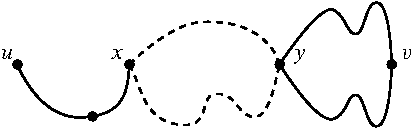
\includegraphics[width=.8\textwidth]{unique-path}

\caption{If there are two paths between $u$ and~$v$, the graph must
  contain a cycle.}

\label{fig:5L}
\end{figure}

\item An additional edge $\edge{u}{v}$ together with the unique path
  between $u$ and $v$ forms a cycle.

\item Suppose that we remove edge $\edge{u}{v}$.  Since the tree
  contained a unique path between $u$ and $v$, that path must have
  been $\edge{u}{v}$.  Therefore, when that edge is removed, no path
  remains, and so the graph is not connected.

\item Let $v_1, \dots, v_m$ be the sequence of vertices on a longest
  path in the tree.  Then $m \geq 2$, since a tree with two vertices
  must contain at least one edge.  There cannot be an edge
  $\edge{v_1}{v_i}$ for $2 < i \leq m$; otherwise, vertices $v_1,
  \dots, v_i$ would from a cycle.  Furthermore, there cannot be
  an edge $\edge{u}{v_1}$ where $u$ is not on the path; otherwise, we
  could make the path longer.  Therefore, the only edge incident to
  $v_1$ is $\edge{v_1}{v_2}$, which means that $v_1$ is a leaf.  By a
  symmetric argument, $v_m$ is a second leaf.

\item We use induction on the number of vertices.  For a tree with a
  single vertex, the claim holds since it has no edges and $0 + 1 = 1$
  vertex.  Now suppose that the claim holds for all $n$-vertex trees
  and consider an $(n+1)$-vertex tree, $T$.  Let $v$ be a leaf of the
  tree.  You can verify that deleting a vertex of degree 1 (and its
  incident edge) from any connected graph leaves a connected subgraph.
  So by~\ref{asub}., deleting $v$ and its incident edge gives a
  smaller tree, and this smaller tree has one more vertex than edge by
  induction.  If we re-attach the vertex, $v$, and its incident edge,
  then the equation still holds because the number of vertices and
  number of edges both increase by 1.  Thus, the claim holds for $T$
  and, by induction, for all trees. \qedhere

\end{enumerate}

\end{proof}

Various subsets of these properties provide alternative characterizations
of trees, though we won't prove this.  For example, a \emph{connected}
graph with a number of vertices one larger than the number of edges is
necessarily a tree.  Also, a graph with unique paths between every pair of
vertices is necessarily a tree.

\subsection{Spanning Trees}

Trees are everywhere.  In fact, every connected graph contains a
subgraph that is a tree with the same vertices as the graph.  This is
a called a \term{spanning tree} for the graph.  For example,
Figure~\ref{fig:5LL} is a connected graph with a spanning tree
highlighted.

\begin{figure}

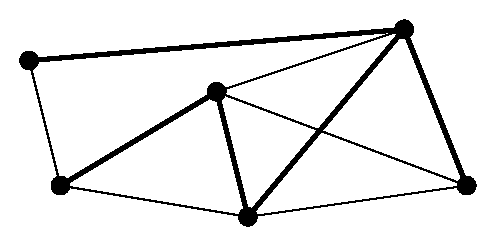
\includegraphics{spanning-tree}

\redrawn

\caption{A graph where the edges of a spanning tree have been
  thickened.}

\label{fig:5LL}

\end{figure}

\begin{theorem}
Every connected graph contains a spanning tree.
\end{theorem}

\begin{proof}
By contradiction.  Assume there is some connected graph~$G$ that has
no spanning tree and let $T$ be a connected subgraph of $G$, with the
same vertices as $G$, and with the smallest number of edges possible
for such a subgraph.  By the assumption, $T$ is not a spanning tree
and so it contains some cycle:
\[
\edge{v_0}{v_1}, \edge{v_1}{v_2}, \dots, \edge{v_k}{v_0}
\]
Suppose that we remove the last edge, $\edge{v_k}{v_0}$.  If a pair of
vertices $x$ and $y$ was joined by a path not containing
$\edge{v_k}{v_0}$, then they remain joined by that path.  On the other
hand, if $x$ and $y$ were joined by a path containing $\edge{v_k}{v_0}$,
then they remain joined by a path containing the remainder of the cycle.
So all the vertices of $G$ are still connected after we remove an edge
from $T$.  This is a contradiction, since $T$ was defined to be a minimum
size connected subgraph with all the vertices of~$G$.  So the theorem
must be true.
\end{proof}

\subsection{Minimum Weight Spanning Trees}

Spanning trees are interesting because they connect all the nodes of a
graph using the smallest possible number of edges.  For example the
spanning tree for the 6-node graph shown in Figure~\ref{fig:5L} has 5
edges.

Spanning trees are very useful in practice, but in the real world, not
all spanning trees are equally desirable.  That's because, in
practice, there are often costs associated with the edge of the graph.

For example, suppose the nodes of a graph represent buildings or towns
and edges represent connections between buildings or towns.  The cost
to actually make a connection may vary a lot from one pair of
buildings or towns to another.  The cost might depend on distance or
topography.  For example, the cost to connect LA to~NY might be much
higher than that to connect NY to Boston.  Or the cost of a pipe
through Manhattan might be more than the cost of a pipe through a
cornfield.

In any case, we typically represent the cost to connect pairs of nodes
with a weighted edge, where the weight of the edge is its cost.  The
weight of a spanning tree is then just the sum of the weights of the
edges in the tree.  For example, the weight of the spanning tree shown
in Figure~\ref{fig:5KA} is~19.

\begin{figure}

\subfloat[]{%
    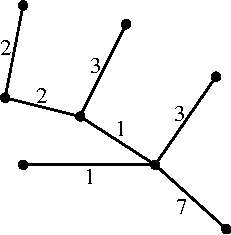
\includegraphics{Fig_5KA-a}
}
%
\qquad
%
\subfloat[]{%
    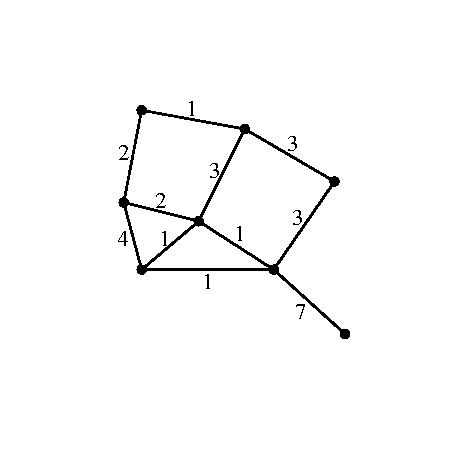
\includegraphics{Fig_5KA-b}
}

\redrawn

\caption{A spanning tree (a) with weight 19 for graph~(b).}

\label{fig:5KA}

\end{figure}

The goal, of course, is to find the spanning tree with minimum weight,
called the min-weight tree (MST for short).

\begin{definition}
The \emph{min-weight spanning tree} \textup(MST\textup) of an
edge-weighted graph~$G$ is the spanning tree of~$G$ with the smallest
possible sum of edge weights.
\end{definition}

Is the spanning tree show in Figure~\ref{fig:5KA}(a) an MST of the
weighted graph shown in Figure~\ref{fig:5KA}(b)?  Actually, it is not,
since the tree shown in Figure~\ref{fig:5KB} is also a spanning tree
of the graph shown in Figure~\ref{fig:5KA}(b), and this spanning tree
has weight~17.

\begin{figure}

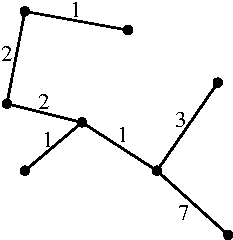
\includegraphics{Fig_5KB}

\redrawn

\caption{An MST for the graph in Figure~\ref{fig:5KA}(b) with
  weight~17.}
\label{fig:5KB}

\end{figure}

What about the graph shown in Figure~\ref{fig:5KB}?  Is it an MST?  It
seems to be, but how do we prove it?  In general, how do we find an
MST\@?  We could, of course, enumerate all trees, but this could take
forever for very large graphs.

Here are two possible algorithms:

\begin{algorithm}\label{alg:MST1}
Grow a tree one edge at a time by adding the minimum weight edge of
the graph to the tree, making sure that you have a tree at each step.
\end{algorithm}

\begin{algorithm}\label{alg:MST2}
\begin{enumerate}

\item Select edges one at a time, always choosing the minimum weight
  edge that does not create a cycle with previously-selected edges.
  We do not impose the constraint that the graph is a tree---our
  selected edges may indeed form a disconnected graph.

\item Continue until we get $n - 1$ edges, i.e., a spanning tree.

\end{enumerate}
\end{algorithm}

For example, in the weighted graph we have been considering, we might
run Algorithm~\ref{alg:MST1} as follows.  We would start by choosing
one of the weight~1 edges, since this is the smallest weight in the
graph.  Suppose we chose the weight~1 edge on the bottom of the
triangle of weight~1 edges in our graph.  This edge is incident to two
weight~1 edges, a weight~4 edge, a weight~7 edge, and a weight~3
edge.  We would then choose the incident edge of minimum weight.  In
this case, one of the two weight~1 edges.  At this point, we cannot
choose the third weight~1 edge since this would form a cycle, but we
can continue by choosing a weight~2 edge.  We might end up with the
spanning tree shown in Figure~\ref{fig:5KC}, which has weight~17, the
smallest we've seen so far.

\begin{figure}

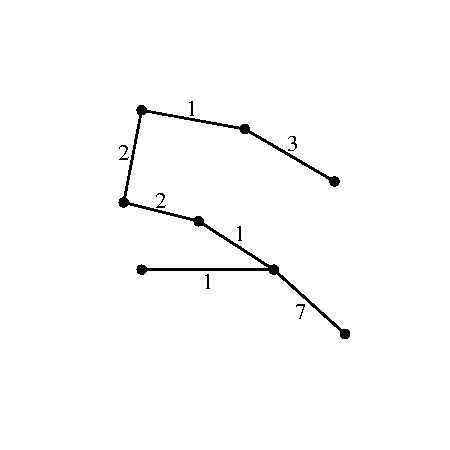
\includegraphics{Fig_5KC}

\redrawn

\caption{A spanning tree found by Algorithm~\ref{alg:MST1}.}

\label{fig:5KC}

\end{figure}

Now suppose we instead ran Algorithm~\ref{alg:MST2} on our graph.  We
might again choose the weight~1 edge on the bottom of the triangle of
weight~1 edges in our graph.  Now, instead of choosing one of the
weight~1 edges it touches, we might choose the weight~1 edge on the
top of the graph.  Note that this edge still has minimum weight, and
does not cause us to form a cycle, so Algorithm~\ref{alg:MST2} can
choose it.  We would then choose one of the remaining weight~1 edges.
Note that neither causes us to form a cycle.  Continuing the
algorithm, we may end up with the same spanning tree in
Figure~\ref{fig:5KC}, though this need not always be the case.

It turns out that both algorithms work, but they might end up with
different MSTs.  The MST is not necessarily unique---indeed, if all
edges of an $n$-node graph have the same weight (${}=1$), then all
spanning trees have weight~$n - 1$.

These are examples of greedy approaches to optimization.  Sometimes it
works and sometimes it doesn't.  The good news is that it works to
find the MST\@.  In fact, both variations work.  It's a little easier
to prove it for Algorithm~\ref{alg:MST2}, so we'll do that one here.

\begin{theorem}\label{thm:MST2}
For any connected, weighted graph~$G$, Algorithm~\ref{alg:MST2}
produces an MST for~$G$.
\end{theorem}

\begin{proof}
The proof is a bit tricky.  We need to show the algorithm terminates,
\ie that if we have selected fewer than $n - 1$ edges, then we can
always find an edge to add that does not create a cycle.  We also need
to show the algorithm creates a tree of minimum weight.

The key to doing all of this is to show that the algorithm never gets
stuck or goes in a bad direction by adding and edge that will keep us
from ultimately producing an MST\@.  The natural way to prove this is
to show that the set of edges selected at any point is contained in
some MST---\ie we can always get to where we need to be.  We'll state
this as a Lemma.

\begin{lemma}\label{lemma:MST2}
For any $m \ge 0$, let $S$ consist of the first $m$ edges selected by
Algorithm~\ref{alg:MST2}.  Then there exists some MST~$T = (V, E)$
for~$G$ such that $S \subseteq E$, \ie the set of edges that we are
growing is always contained in some MST\@.
\end{lemma}

We'll prove this momentarily, but first let's see why it helps prove
the theorem.  Assume the lemma is true.  Then how do we know
Algorithm~\ref{alg:MST2} can always find an edge to add without
creating a cycle?  Well, as long as there are fewer than $n - 1$ edges
picked, there exists some edge in $E - S$ and so there is an edge that
we can add to~$S$ without forming a cycle.  Next, how do we know that
we get an MST at the end?  Well, once $m = n - 1$, we know that $S$ is
an MST\@.

Ok, so the theorem is an easy corollary of the lemma.  To prove the
lemma, we'll use induction on the number of edges chosen by the
algorithm so far.  This is very typical in proving that an algorithm
preserves some kind of invariant condition---induct on the number of
steps taken, \ie the number of edges added.

Our inductive hypothesis $P(m)$ is the following: for any $G$ and any
set~$S$ of $m$ edges initially selected by Algorithm~\ref{alg:MST2},
there exists an MST $T = (V, E)$ of~$G$ such that $S \subseteq E$.

For the base case, we need to show $P(0)$.  In this case $S =
\emptyset$, so $S \subseteq E$ trivially holds for any MST $T = (V,
E)$.

For the inductive step, we assume $P(m)$ holds and we show that it
implies $P(m + 1)$.  Let $e$ denote the $(m+1)$st edge selected by
Algorithm~\ref{alg:MST2}, and let $S$ denote the first $m$ edges
selected by Algorithm~\ref{alg:MST2}.  Let $T^* = (V^*, E^*)$ be the
MST such that $S \subseteq E*$, which exists by the inductive
hypothesis.  There are now two cases:
\begin{description}

\item[Case 1:]
$e \in E^*$, in which case $S \union \{e\} \subseteq E^*$, and thus
  $P(m+1)$ holds.

\item[Case 2:]
$e \notin E^*$, as illustrated in Figure~\ref{fig:5KD}.  Now we need
  to find a different MST that contains $S$ and~$e$.

\begin{figure}

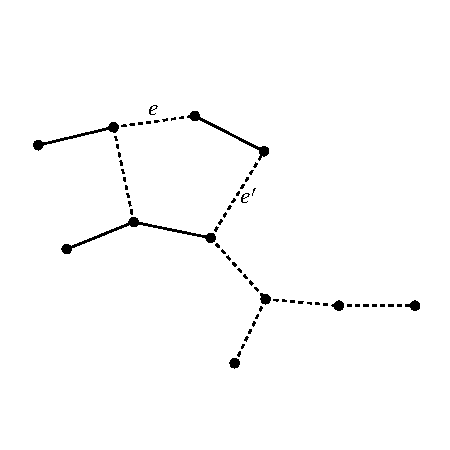
\includegraphics{Fig_5KD}

\redrawn

\caption{The graph formed by adding $e$ to $T^*$.  Edges of~$S$ are
  denoted with solid lines and edges of $E^* - S$ are denoted with
  dashed lines.}

\label{fig:5KD}
\end{figure}

\end{description}

What happens when we add $e$ to~$T^*$?  Since $T^*$ is a tree, we get
a cycle.  (Here we used part~3 of Theorem~\ref{th:treeprops}.)
Moreover, the cycle cannot only contains edges in~$S$, since $e$ was
chosen so that together with the edges in~$S$, it does not form a
cycle.  This implies that $\{e\} \union T^*$ contains a cycle that
contains an edge $e'4$ of $E^* - S$.  For example, such an $e'$ is
shown in Figure~\ref{fig:5KD}.

Note that the weight of~$e$ is at most that of~$e'$.  Indeed,
Algorithm~\ref{alg:MST2} picks the minimum weight edge that does not
make a cycle with~$S$.  Since $e' \in T^*$, it cannot make a cycle
with~$S$.

Okay, we're almost done.  Now we'll make an MST that contains $S
\union \{e\}$.  Let $T^{**} = (V, E^{**})$ where $E^{**} = (E^* -
\{e'\}) \union \{e\}$, that is, we swap $e$ and~$e'$ in~$T^*$.

\begin{claim}\label{claim:MST2}
$T^{**}$ is an MST.
\end{claim}

\begin{proof}[Proof of claim]
We first show that $T^{**}$ is a spanning tree.  
$T^{**}$ is acyclic
because it was produced by removing an edge from the only cycle in
$T^{*} \union \{e\}$.
$T^{**}$ is connected
since the edge we deleted from $T^* \union \{e\}$ was on a cycle.
It follows by Theorem~\ref{thm:???} that $T^{**}$ is a spanning tree.

Now let's look at the weight of~$T^{**}$.  Well, since the weight
of~$e$ was at most that of~$e'$, the weight of~$T^{**}$ is at most
that of~$T^*$, and thus $T^{**}$ is an MST\@
\end{proof}

Since $S \union \{e\} \subseteq E^{**}$, $P(m + 1)$ holds.  Thus, when
Algorithm~\ref{alg:MST2} has $n - 1$ edges, it produces an MST\@.
\end{proof}

So now we know for sure that the MST for our example graph has
weight~17 since it was produced by Algorithm~\ref{alg:MST2}.  And we
have a fast algorithm for finding a minimum-weight spanning tree for
any graph.

%% Trees Problems %%%%%%%%%%%%%%%%%%%%%%%%%%%%%%%%%%%%%%%%%%%%%%%%%%%%%%%%%%%%%
\begin{problems}
\classproblems
\pinput{CP_graph_edge_mark}
\pinput{CP_spanning_tree_proc}
\pinput{CP_tree_characterizations}
%\pinput{CP_23_high_priority_servers}

\homeworkproblems
\pinput{PS_average_degree_of_tree_and_simple_path}
% S09.cp6t.2
% S09.cp6t.3
\end{problems}


%% Coloring Graphs Problems %%%%%%%%%%%%%%%%%%%%%%%%%%%%%%%%%%%%%%%%%%%%%%%%%%%
\begin{problems}
\classproblems
\pinput{CP_chromatic_number}

% S09.cp6r.1
% S09.cp6r.2

\homeworkproblems
\pinput{PS_TA_recitation_graph_coloring}
\pinput{PS_graph_colorable}
%\pinput{PS_simple_triangle_free_graph_coloring}

\examproblems
\pinput{FP_coloring_false_proof}

\end{problems}

%% Bipartite Matchings Problems %%%%%%%%%%%%%%%%%%%%%%%%%%%%%%%%%%%%%%%%%%%%%%%
% S09.cp6r.3
% S09.cp6r.4

\begin{problems}
\classproblems
\pinput{CP_student_clubs}
\pinput{CP_latin_squares}

\examproblems
\pinput{MQ_bipartite-matching_recitations}

\homeworkproblems
\pinput{PS_no_odd_length_cycles}
\pinput{PS_cards_in_4_rows_13_columns}
\pinput{PS_bipartite_matching_virtues}
\end{problems}

\section{Planar Graphs}\label{planar_graphs_sec}

\subsection{Drawing Graphs in the Plane}

Suppose there are three dogs and three houses, as shown in
Figure~\ref{fig:5DP}.  Can you find a route from each dog to each
house such that no route crosses any other route?

\begin{figure}[h]

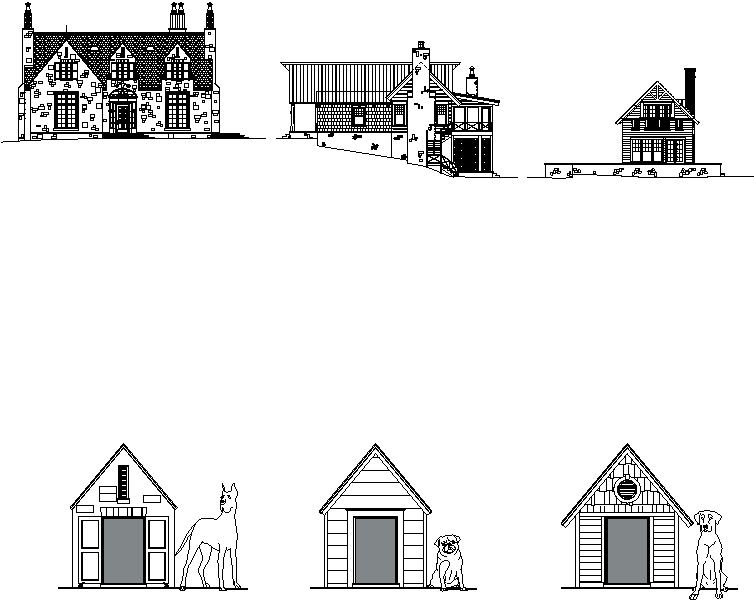
\includegraphics{dog-houses}

\redrawn

\caption{Three dogs and three houses.  Is there a route from each dog
  to each house so that no pair of the 9 routes cross each other?}
\label{fig:5DP}
\end{figure}

A \emph{quadrapus} is a little-known animal similar to an octopus, but
with four arms.  Suppose there are five quadrapi resting on the sea
floor, as shown in Figure~\ref{fig:5DA}.  Can each quadrapus
simultaneously shake hands with every other in such a way that no arms
cross?

\begin{figure}

%\mfigure{!}{2in}{quadrapi}

\setlength{\unitlength}{2000sp}%{3947sp}%
%
\begingroup\makeatletter\ifx\SetFigFont\undefined%
\gdef\SetFigFont#1#2#3#4#5{%
  \reset@font\fontsize{#1}{#2pt}%
  \fontfamily{#3}\fontseries{#4}\fontshape{#5}%
  \selectfont}%
\fi\endgroup%
\begin{picture}(11049,5049)(589,-5248)
{\color[rgb]{0,0,0}%\thinlines
\put(4688,-1673){\oval(524,524)}
}%
{\color[rgb]{0,0,0}\put(1913,-2948){\oval(524,524)}
}%
{\color[rgb]{0,0,0}\put(4538,-3923){\oval(524,524)}
}%
{\color[rgb]{0,0,0}\put(7838,-3098){\oval(524,524)}
}%
{\color[rgb]{0,0,0}\put(9713,-1748){\oval(524,524)}
}%
{\color[rgb]{0,0,0}\put(4426,-1636){\line(-1, 0){900}}
\multiput(3526,-1636)(-2.67857,-8.03571){57}{\makebox(1.6667,11.6667){\SetFigFont{5}{6}{\rmdefault}{\mddefault}{\updefault}.}}
\put(3376,-2086){\line(-1, 0){750}}
}%
{\color[rgb]{0,0,0}\put(4951,-1711){\line( 5,-3){893.382}}
\put(5851,-2236){\line( 5, 6){442.623}}
\put(6301,-1711){\line( 2,-3){300}}
}%
{\color[rgb]{0,0,0}\multiput(1876,-2686)(1.37838,8.27027){101}{\makebox(1.6667,11.6667){\SetFigFont{5}{6}{\rmdefault}{\mddefault}{\updefault}.}}
\put(2026,-1861){\line( 5, 2){685.345}}
\put(2701,-1561){\line( 0, 1){375}}
}%
{\color[rgb]{0,0,0}\put(2176,-2986){\line( 5, 2){750}}
\put(2926,-2686){\line( 5,-6){510.246}}
\put(3451,-3286){\line( 6, 1){450}}
}%
{\color[rgb]{0,0,0}\put(1951,-3211){\line(-1,-2){300}}
\put(1651,-3811){\line( 5,-6){375}}
\put(2026,-4261){\line( 3, 2){450}}
}%
{\color[rgb]{0,0,0}\put(1651,-2986){\line(-6, 5){612.295}}
\put(1051,-2461){\line(-5,-6){442.623}}
\multiput(601,-2986)(2.02703,-8.10811){75}{\makebox(1.6667,11.6667){\SetFigFont{5}{6}{\rmdefault}{\mddefault}{\updefault}.}}
}%
{\color[rgb]{0,0,0}\multiput(4501,-3661)(1.37838,8.27027){101}{\makebox(1.6667,11.6667){\SetFigFont{5}{6}{\rmdefault}{\mddefault}{\updefault}.}}
\put(4651,-2836){\line( 5, 2){685.345}}
\put(5326,-2536){\line( 0, 1){375}}
}%
{\color[rgb]{0,0,0}\put(4801,-3961){\line( 5, 2){750}}
\put(5551,-3661){\line( 5,-6){510.246}}
\put(6076,-4261){\line( 6, 1){450}}
}%
{\color[rgb]{0,0,0}\put(4576,-4186){\line(-1,-2){300}}
\put(4276,-4786){\line( 5,-6){375}}
\put(4651,-5236){\line( 3, 2){450}}
}%
{\color[rgb]{0,0,0}\put(7576,-3061){\line(-1, 0){900}}
\multiput(6676,-3061)(-2.67857,-8.03571){57}{\makebox(1.6667,11.6667){\SetFigFont{5}{6}{\rmdefault}{\mddefault}{\updefault}.}}
\put(6526,-3511){\line(-1, 0){750}}
}%
{\color[rgb]{0,0,0}\put(7876,-2836){\line(-1, 1){375}}
\put(7501,-2461){\line( 4, 3){600}}
\put(8101,-2011){\line( 0, 1){450}}
}%
{\color[rgb]{0,0,0}\put(8101,-3136){\line( 5,-3){893.382}}
\put(9001,-3661){\line( 5, 6){442.623}}
\put(9451,-3136){\line( 2,-3){300}}
}%
{\color[rgb]{0,0,0}\put(7876,-3361){\line(-2,-5){237.931}}
\put(7651,-3961){\line( 1,-1){600}}
}%
{\color[rgb]{0,0,0}\put(9751,-1486){\line(-1, 1){375}}
\put(9376,-1111){\line( 4, 3){600}}
\put(9976,-661){\line( 0, 1){450}}
}%
{\color[rgb]{0,0,0}\put(9976,-1786){\line( 5,-3){893.382}}
\put(10876,-2311){\line( 5, 6){442.623}}
\put(11326,-1786){\line( 2,-3){300}}
}%
{\color[rgb]{0,0,0}\put(9751,-2011){\line(-2,-5){237.931}}
\put(9526,-2611){\line( 1,-1){600}}
}%
{\color[rgb]{0,0,0}\put(9451,-1711){\line(-5,-1){677.885}}
\put(8776,-1861){\line(-2, 3){692.308}}
\put(8101,-811){\line(-5,-1){1572.115}}
}%
{\color[rgb]{0,0,0}\put(4651,-1936){\line(-1,-4){339.706}}
\put(4276,-3286){\line(-4,-1){1358.823}}
\multiput(2926,-3661)(-1.37838,-8.27027){101}{\makebox(1.6667,11.6667){\SetFigFont{5}{6}{\rmdefault}{\mddefault}{\updefault}.}}
}%
{\color[rgb]{0,0,0}\put(4276,-3886){\line(-3,-2){761.538}}
\multiput(3526,-4411)(2.03287,-8.13149){103}{\makebox(1.6667,11.6667){\SetFigFont{5}{6}{\rmdefault}{\mddefault}{\updefault}.}}
}%
{\color[rgb]{0,0,0}\multiput(4726,-1411)(-1.37387,8.24324){91}{\makebox(1.6667,11.6667){\SetFigFont{5}{6}{\rmdefault}{\mddefault}{\updefault}.}}
\put(4651,-661){\line( 2,-1){1290}}
\put(5926,-1336){\line( 6,-1){1277.027}}
}%
\end{picture}%


\caption{Five quadrapi (4-armed creatures).}

\label{fig:5DA}

\end{figure}

\begin{staffnotes}
rephrased by ARM 7/3/10:
\end{staffnotes}

A \emph{\idx{planar graph}} is a graph that can be drawn in the place so
that no nodes or edges overlap and so that no edges cross each other.
Thus, these two puzzles are asking whether the graphs in
Figure~\ref{fig:nonplanar} are planar; that is, whether they can be
redrawn so that no edges cross.  The first graph is called the
\term{complete bipartite graph}, \idx{$K_{3,3}$}, and the second is
\idx{$K_5$}.
\begin{figure}
%\mfigure{!}{1.5in}{nonplanar}
\setlength{\unitlength}{3000sp}%{3947sp}%
%
\begingroup\makeatletter\ifx\SetFigFont\undefined%
\gdef\SetFigFont#1#2#3#4#5{%
  \reset@font\fontsize{#1}{#2pt}%
  \fontfamily{#3}\fontseries{#4}\fontshape{#5}%
  \selectfont}%
\fi\endgroup%
\begin{picture}(7366,2266)(2318,-2244)
{\color[rgb]{0,0,0}%\thinlines
\put(2401,-661){\circle{150}}
}%
{\color[rgb]{0,0,0}\put(4726,-661){\circle{150}}
}%
{\color[rgb]{0,0,0}\put(3601,-661){\circle{150}}
}%
{\color[rgb]{0,0,0}\put(3601,-2161){\circle{150}}
}%
{\color[rgb]{0,0,0}\put(2401,-2161){\circle{150}}
}%
{\color[rgb]{0,0,0}\put(4801,-2161){\circle{150}}
}%
{\color[rgb]{0,0,0}\put(8401,-61){\circle{150}}
}%
{\color[rgb]{0,0,0}\put(7201,-961){\circle{150}}
}%
{\color[rgb]{0,0,0}\put(9601,-961){\circle{150}}
}%
{\color[rgb]{0,0,0}\put(7801,-2161){\circle{150}}
}%
{\color[rgb]{0,0,0}\put(9001,-2161){\circle{150}}
}%
{\color[rgb]{0,0,0}\put(2401,-661){\line( 0,-1){1500}}
\put(2401,-2161){\line( 4, 5){1200}}
\put(3601,-661){\line( 4,-5){1200}}
\put(4801,-2161){\line( 0, 1){1500}}
\put(4726,-661){\line(-3,-4){1125}}
\put(3601,-2161){\line(-4, 5){1200}}
}%
{\color[rgb]{0,0,0}\put(3601,-661){\line( 0,-1){1500}}
}%
{\color[rgb]{0,0,0}\put(2401,-661){\line( 5,-3){2426.471}}
}%
{\color[rgb]{0,0,0}\put(4726,-661){\line(-3,-2){2301.923}}
}%
{\color[rgb]{0,0,0}\put(7201,-961){\line( 1,-2){600}}
\put(7801,-2161){\line( 1, 0){1200}}
\put(9001,-2161){\line( 1, 2){600}}
\put(9601,-961){\line(-4, 3){1200}}
\put(8401,-61){\line(-4,-3){1200}}
\put(7201,-961){\line( 1, 0){2400}}
\put(9601,-961){\line(-3,-2){1800}}
\put(7801,-2161){\line( 1, 4){529.412}}
\put(8401,-61){\line( 1,-4){529.412}}
}%
{\color[rgb]{0,0,0}\put(9001,-2161){\line(-3, 2){1800}}
}%
\end{picture}%

\caption{$K_{3, 3}$ (a) and $K_5$ (b).  Can you redraw these graphs so
that no pairs of edges cross?}
\label{fig:nonplanar}
\end{figure}

In each case, the answer is, ``No ---but almost!''  In fact, if you
remove an edge from either of them, then the resulting graphs
\emph{can} be redrawn in the plane so that no edges cross.  For
example, we have illustrated the planar drawings for each resulting
graph in Figure~\ref{fig:5DC}.

\begin{figure}

\missinggraphic

\caption{Planar drawings of $K_{3, 3} - \{ u, v \}$ (a) and $K_5 - \{
  u, v \}$ (b).}
\label{fig:5DC}
\end{figure}

Planar drawings have applications in circuit layout and are helpful in
displaying graphical data such as program flow charts, organizational
charts, and scheduling conflicts. For these applications, the goal is
to draw the graph in the plane with as few edge crossings as possible.
(See the box on the following page for one such example.)

\begin{figure}
\textbox{\noindent
When wires are arranged on a surface, like a circuit board or microchip,
crossings require troublesome three-dimensional structures.  When Steve
Wozniak designed the disk drive for the early Apple II computer, he
struggled mightily to achieve a nearly planar design:
%
\begin{quotation}
\noindent For two weeks, he worked late each night to make a satisfactory
design.  When he was finished, he found that if he moved a connector he
could cut down on feedthroughs, making the board more reliable.  To make
that move, however, he had to start over in his design.  This time it only
took twenty hours. He then saw another feedthrough that could be
eliminated, and again started over on his design.  ``The final design was
generally recognized by computer engineers as brilliant and was by
engineering aesthetics beautiful.  Woz later said, 'It's something you can
only do if you're the engineer and the PC board layout person yourself.
That was an artistic layout.  The board has virtually no
feedthroughs.'\,''\footnote{From apple2history.org which in turn quotes
\textit{Fire in the Valley} by Freiberger and Swaine.}
\end{quotation}
}
\end{figure}

\subsection{A Recursive Definition for Planar Graphs}\label{sec:recdef_planar}

We've taken the meaning of planar drawings for granted up till now,
but if we're going to \emph{prove} things about planar graphs, we
better have a precise definition.

\begin{definition}\label{def:planar_graph}
A \term{drawing} of a graph assigns to each node a distinct point in
the plane and assigns to each edge a smooth curve in the plane whose
endpoints correspond to the nodes incident to the edge.  The drawing
is \index{planar drawing}\emph{planar} if none of the curves
\emph{cross} themselves or other curves, namely, the only points that
appear more than once on any of the curves are the node points.  A
graph is \index{planar graph}\emph{planar} when it has a planar
drawing.
\end{definition}

Definition~\ref{def:planar_graph} is precise but takes for granted
further concepts: ``smooth planar curves'' and ``points appearing more
than once'' on them.  We haven't defined these concepts ---we just
showed the simple picture in Figure~\ref{fig:5DC} and hoped you would
get the idea.

Pictures can be a great way to get a new idea across, but it is
generally not a good idea to assume a picture can replace precise
mathematics.  Relying solely on pictures can sometimes lead to
disaster ---or to false proofs, anyway.  There is a long history of
false proofs about planar graphs based on misleading
pictures.\footnote{\textcolor{red}{XYZ's} false proof of the 4-Color
  Theorem for planar graphs is not the only example.  Mistakes creep
  in with statements like,
\begin{quote}
    As you can see from Figure~ABC, it must be that property~XYZ holds
    for all planar graphs.
\end{quote}}

Working with planar drawings in a precise way would take a
chapter-long excursion into continuous mathematics just to develop the
needed concepts from plane geometry and topology.  So
Definition~\ref{def:planar_graph} is troublesome for us to use.  The
good news is that there is another way to define planar graphs that
uses only discrete mathematics.  In particular, we can define planar
graphs as a recursive data type.  In order to understand how it works,
we first need to understand the concept of a \emph{face} in a planar
drawing.

\subsubsection{Faces}

In a planar drawing of a graph. the curves corresponding to the edges
divide up the plane into connected regions.  These regions are called
the \term{continuous faces}\footnote{Most texts drop the adjective
  \emph{continuous} from the definition of a face as a connected
  region.  We need the adjective to distinguish a continuous face from
  the the \emph{discrete} face which describes the closed walk
  corresponding to node points along the boundary of the continuous
  face.}  For example, the drawing in
Figure~\ref{fig:continuous-faces} has four continuous faces.  Face IV,
which extends off to infinity in all directions, is called the
\term{outside face}.

\begin{figure}[h]
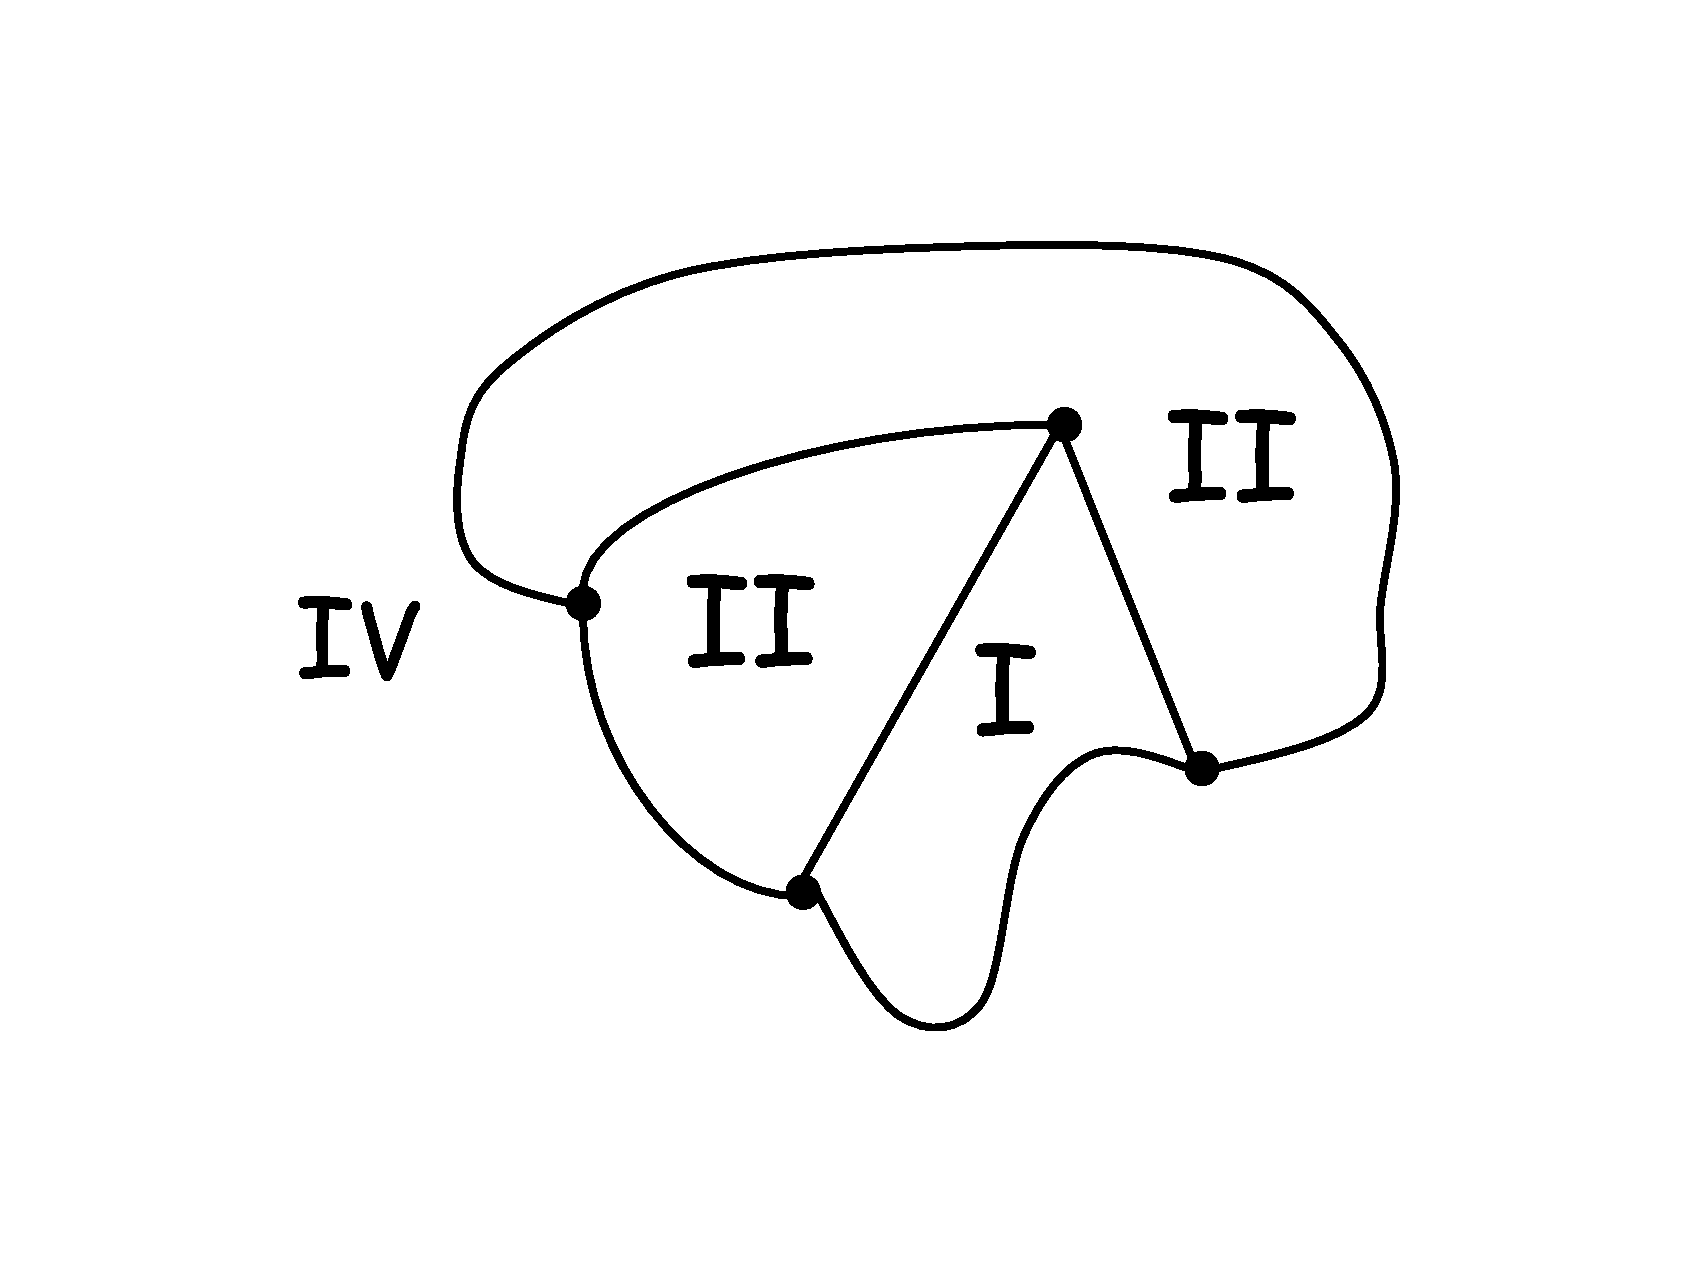
\includegraphics[height=2in]{continuous-faces}
\missinggraphic[Fix label of region III]
\caption{A planar drawing with four faces.}
\label{fig:continuous-faces}
\end{figure}

The vertices along the boundary of each face in
Figure~\ref{fig:continuous-faces} form a cycle.  For example, labeling
the vertices as in Figure~\ref{fig:continuous-cycles}, the cycles for
the face boundaries are
\begin{equation}\label{eq:5DA}
\mathtt{abca}\qquad \mathtt{abda}\qquad \mathtt{bcdb}\qquad \mathtt{acda}.
\end{equation}
These four cycles correspond nicely to the four continuous faces in
Figure~\ref{fig:continuous-cycles} ---so nicely, in fact, that we can
identify each of the faces in Figure~\ref{fig:continuous-cycles} by
its cycle.  For example, the cycle \texttt{abca} identifies
face~III\@.  The cycles in list~\ref{eq:5DA} are called the
\emph{discrete faces} of the graph in
Figure~\ref{fig:continuous-cycles}.  We use the term ``discrete''
since cycles in a graph are a discrete data type ---as opposed to a
region in the plane, which is a continuous data type.

\begin{figure}
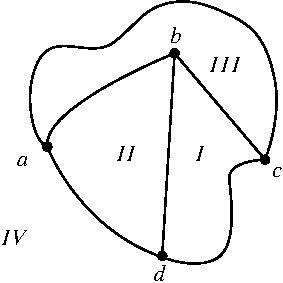
\includegraphics[height=2in]{continuous-cycles}
\caption{The drawing with labelled vertices.}
\label{fig:continuous-cycles}
\end{figure}

Unfortunately, continuous faces in planar drawings are not always
bounded by cycles in the graph ---things can get a little more
complicated.  For example, the planar drawing in
Figure~\ref{fig:bridge} has what we will call a \emph{bridge}, namely,
the edge $\edge{c}{e}$.  The sequence of vertices along the boundary
of the outer region of the drawing is
\[
\mathtt{abcefgecda}.
\]
This sequence defines a closed walk, but does not define a cycle since
the walk traverses the bridge $\edge{c}{e}$ twice.

\begin{figure}[h]
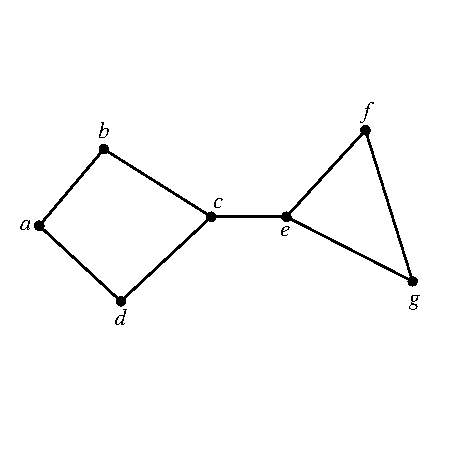
\includegraphics[height=2in]{edge-twice-same-face}
\caption{A planar drawing with a \emph{bridge}.}
\label{fig:bridge}
\end{figure}

The planar drawing in Figure~\ref{fig:dongle} illustrates another
complication.  This drawing has what we will call a \emph{dongle},
namely, the nodes $v$, $x$, $y$, and~$w$, and the edges incident to
them.  The sequence of vertices along the boundary
of the inner region is
\[
\mathtt{rstvxyxvwvtur}.
\]
This sequence defines a closed walk, but once again does not define a
cycle, because the walk traverses \emph{every} edge of the dongle twice
---once ``coming'' and once ``going.''

\begin{figure}[h]
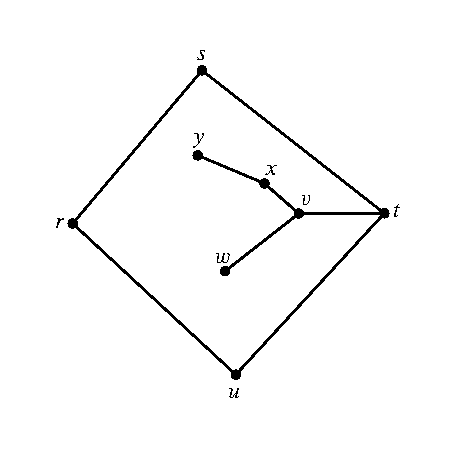
\includegraphics[height=2in]{dongle-face}
\caption{A planar drawing with a \emph{dongle}.}
\label{fig:dongle}
\end{figure}

It turns out that bridges and dongles are the only complications, at
least for connected graphs.  In particular, every continuous face in a
planar drawing corresponds to a closed walk in the graph.  We refer to
such closed walks as the \emph{discrete faces} of the drawing.

\subsubsection{A Recursive Definition for Planar Embeddings}

The association between the continuous faces of a planar drawing and
closed walks will allow us to characterize a planar drawing in terms
of the closed walks that bound the continuous faces.  In particular,
it leads us to the discrete data type of \term{planar embeddings} that
we can use in place of continuous planar drawings.  Namely, we'll
define a planar embedding recursively to be the set of
boundary-tracing closed walks we could get by drawing one edge after
another.

\begin{definition}\label{def:embedding}\label{embeddingdef}
A \term{planar embedding} of a \emph{connected} graph consists of a
nonempty set of closed walks of the graph called the \term{discrete
  faces} of the embedding.  Planar embeddings are defined recursively
as follows:

\inductioncase{Base case}: If $G$ is a graph consisting of a single
vertex, $v$, then a planar embedding of $G$ has one discrete face,
namely the length zero closed walk, $v$.

\inductioncase{Constructor Case} (split a face): Suppose $G$ is a
connected graph with a planar embedding, and suppose $a$ and $b$ are
distinct, nonadjacent vertices of $G$ that appear on some discrete
face, $\gamma$, of the planar embedding.  That is, $\gamma$ is a
closed walk of the form
\[
a \dots b \cdots a.
\]
Then the graph obtained by adding the edge $\edge{a}{b}$ to the edges
of $G$ has a planar embedding with the same discrete faces as $G$,
except that face $\gamma$ is replaced by the two discrete
faces\footnote{\label{C} There is a special case of this rule.  If $G$
  is a line graph beginning with $a$ and ending with $b$, then the
  cycles into which $\gamma$ splits are actually the same.  That's
  because adding edge $\edge{a}{b}$ creates a simple cycle graph,
  $C_n$, that divides the plane into an ``inner'' and an ``outer''
  region with the same border.  In order to maintain the
  correspondence between continuous faces and discrete faces, we have
  to allow two ``copies'' of this same cycle to count as discrete
  faces.}
\[
a\dots ba\quad \text{ and } \quad ab\cdots a,
\]
as illustrated in Figure~\ref{fig:face-splitting}.

\begin{figure}[h]
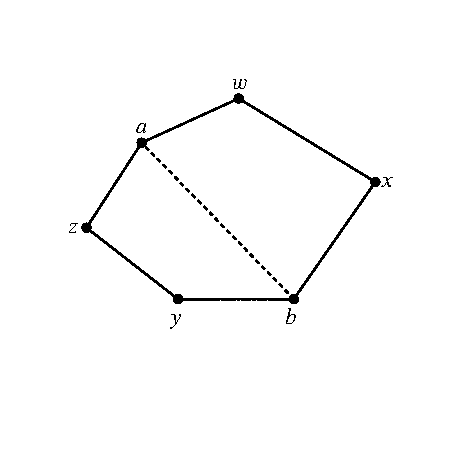
\includegraphics[height=2.5in]{split-a-face}
\caption{The ``split a face'' case.}
\label{fig:face-splitting}
\end{figure}

\inductioncase{Constructor Case} (add a bridge): Suppose $G$ and~$H$
are connected graphs with planar embeddings and disjoint sets of
vertices.  Let $a$ be a vertex on a discrete face, $\gamma$, in the
embedding of $G$.  That is, $\gamma$ is of the form
\[
a\dots a.
\]
Similarly, let $b$ be a vertex on a discrete face, $\delta$, in the
embedding of $H$, so $\delta$ is of the form
\[
b\cdots b.
\]
Then the graph obtained by connecting $G$ and $H$ with a new edge,
$\edge{a}{b}$, has a planar embedding whose discrete faces are the union of
the discrete faces of $G$ and $H$, except that faces $\gamma$ and $\delta$
are replaced by one new face
\[
a\dots ab\cdots ba.
\]
This is illustrated in Figure~\ref{fig:add-bridge}, where the faces of
$G$ and $H$ are:
\[
G: \set{\texttt{axyza},\ \texttt{axya},\ \texttt{ayza}}
    \qquad H: \set{\texttt{btuvwb},\ \texttt{btvwb},\ \texttt{tuvt}},
\]
and after adding the bridge $\edge{\texttt{a}}{\texttt{b}}$, there is a
single connected graph with faces
\[
\set{\texttt{axyz{\color{blue}ab}tuvw{\color{blue}ba}},\
         \texttt{axya},\ \texttt{ayza},\ \texttt{btvwb},\ \texttt{tuvt}}.
\]

\begin{figure}[h]
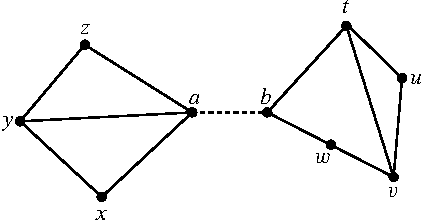
\includegraphics[height=3in]{add-bridge}
\caption{The ``add a bridge'' case.}
\label{fig:add-bridge}
\end{figure}

\end{definition}

\subsubsection{Does It Work?}

Yes!  In general, a graph is planar if and only if each of its
connected components has a planar embedding as defined in
Definition~\ref{def:embedding}.  Unfortunately, proving this fact
requires a bunch of mathematics that we don't cover in this
text---stuff like geometry and topology.  Of course, that is why we
went to the trouble of including Definition~\ref{def:embedding}---we
don't want to deal with that stuff in this text and now that we have a
recursive definition for planar graphs, we won't need to.  That's the
good news.

The bad news is that Definition~\ref{def:embedding} looks a lot more
complicated than the intuitively simple notion of a drawing where
edges don't cross.  It seems like it would be easier to stick to the
simple notion and give proofs using pictures.  Perhaps so, but your
proofs are more likely to be complete and correct if you work from the
discrete Definition~\ref{def:embedding} instead of the continuous
Definition~\ref{def:planar_graph}.

\subsubsection{Where Did the Outer Face Go?}

Every planar drawing has an immediately-recognizable outer face---its
the one that goes to infinity in all directions.  But where is the
outer face in a planar embedding?

There isn't one!  That's because there really isn't any need to
distinguish one.  In fact, a planar embedding could be drawn with any
given face on the outside.  An intuitive explanation of this is to
think of drawing the embedding on a \emph{sphere} instead of the
plane.  Then any face can be made the outside face by ``puncturing''
that face of the sphere, stretching the puncture hole to a circle
around the rest of the faces, and flattening the circular drawing onto
the plane.

So pictures that show different ``outside'' boundaries may actually be
illustrations of the same planar embedding.  For example, the two
embeddings shown in Figure~\ref{fig:5DE} are really the same.

\begin{figure}
\missinggraphic
\caption{Two illustrations of the same embedding.}
\label{fig:5DE}
\end{figure}

This is what justifies the ``add bridge'' case in a planar embedding:
whatever face is chosen in the embeddings of each of the disjoint planar
graphs, we can draw a bridge between them without needing to cross any
other edges in the drawing, because we can assume the bridge connects
two ``outer'' faces.

\subsection{Euler's Formula}

The value of the recursive definition is that it provides a powerful
technique for proving properties of planar graphs, namely, structural
induction.  For example, we will now use
Definition~\ref{def:embedding} and structural induction to establish
one of the most basic properties of a connected planar graph; namely,
the number of vertices and edges completely determines the number of
faces in every possible planar embedding of the graph.

\begin{theorem}[\idx{Euler's Formula}]\label{thm:eulers_formula}
If a connected graph has a planar embedding, then
\begin{equation*}
    v - e + f = 2
\end{equation*}
where $v$ is the number of vertices, $e$ is the number of edges, and
$f$ is the number of faces.
\end{theorem}

For example, in Figure~\ref{fig:continuous-faces}, $\card{V} = 4$,
$\card{E} = 6$, and $f = 4$.  Sure enough, $4 - 6 + 4 = 2$, as Euler's
Formula claims.

\begin{proof}
The proof is by structural induction on the definition of planar
embeddings.  Let $P(\embed{E})$ be the proposition that $v - e + f = 2$ for an
embedding, $\embed{E}$.

\inductioncase{Base case}: ($\embed{E}$ is the one-vertex planar
embedding).  By definition, $v=1$, $e=0$, and $f=1$, so $P(\embed{E})$
indeed holds.

\inductioncase{Constructor case} (split a face): Suppose $G$ is a
connected graph with a planar embedding, and suppose $a$ and $b$ are
distinct, nonadjacent vertices of $G$ that appear on some discrete
face, $\gamma= a \dots b \cdots a$, of the planar embedding.

Then the graph obtained by adding the edge $\edge{a}{b}$ to the edges of
$G$ has a planar embedding with one more face and one more edge than $G$.
So the quantity $v-e+f$ will remain the same for both graphs, and since by
structural induction this quantity is 2 for $G$'s embedding, it's also 2
for the embedding of $G$ with the added edge.  So $P$ holds for the
constructed embedding.

\inductioncase{Constructor case} (add bridge): Suppose $G$ and $H$ are
connected graphs with planar embeddings and disjoint sets of vertices.
Then connecting these two graphs with a bridge merges the two bridged
faces into a single face, and leaves all other faces unchanged.  So
the bridge operation yields a planar embedding of a connected graph
with $v_G +v_H$ vertices, $e_G + e_H +1$ edges, and $f_G + f_H - 1$
faces.  Since
\begin{align*}
\lefteqn{(v_G +v_H) - (e_G + e_H +1) + (f_G + f_H - 1)} \qquad\\
   & = (v_G  - e_G + f_G) + (v_H  - e_H  + f_H) -2\\
   & = (2)+(2)-2 & \text{(by structural induction hypothesis)}\\
   & = 2,
\end{align*}
$v-e+f$ remains equal to~2 for the constructed embedding.  That is,
$P$ also holds in this case.

This completes the proof of the constructor cases, and the theorem follows
by structural induction.
\end{proof}

\subsection{Bounding the Number of Edges in a Planar Graph}

Like Euler's formula, the following lemmas follow by structural induction
directly from Definition~\ref{def:embedding}.

\begin{lemma}\label{2e}
In a planar embedding of a connected graph, each edge is traversed once by
each of two different faces, or is traversed exactly twice by one face.
\end{lemma}

\begin{lemma}\label{3f}
  In a planar embedding of a connected graph with at least three vertices,
  each face is of length at least three.
\end{lemma}

Combining Lemmas~\ref{2e} and~\ref{3f} with Euler's Formula, we can
now prove that planar graphs have a limited number of edges:

\begin{theorem}\label{e3v}
Suppose a connected planar graph has $v \geq 3$ vertices and $e$ edges.
Then
\begin{equation*}
    e \leq 3v-6.
\end{equation*}
\end{theorem}

\begin{proof}
By definition, a connected graph is planar iff it has a planar embedding.
So suppose a connected graph with $v$ vertices and $e$ edges has a planar
embedding with $f$ faces.  By Lemma~\ref{2e}, every edge is traversed
exactly twice by the face boundaries.  So the sum of the lengths of the
face boundaries is exactly $2e$.  Also by Lemma~\ref{3f}, when $v \geq 3$,
each face boundary is of length at least three, so this sum is at least
$3f$.  This implies that
\begin{equation}\label{e3f}
3f \leq 2e.
\end{equation}
But $f = e-v+2$ by Euler's formula, and substituting into~\eqref{e3f} gives
\begin{align*}
3(e-v+2) & \leq 2e\\
e-3v + 6  & \leq 0\\
e & \leq 3v - 6 \qedhere
\end{align*}
\end{proof}

\section{Returning to $K_5$ and $K_{3,3}$}

Theorem~\ref{e3v} lets us prove that the quadrapi can't all shake hands
without crossing.  Representing quadrapi by vertices and the necessary
handshakes by edges, we get the complete graph, \idx{$K_5$}.  Shaking
hands without crossing amounts to showing that $K_5$ is planar.  But
$K_5$ is connected, has 5 vertices and 10 edges, and $10 > 3 \cdot
5-6$.  This violates the condition of Theorem~\ref{e3v} required for
$K_5$ to be planar, which proves
\begin{corollary}\label{k5not}
$K_5$ is not planar.
\end{corollary}

We can also use Euler's Formula to show that $K_{3, 3}$ is not
planar.  The proof is similar to that of Theorem~\ref{e3v} except that
we use the additional fact that $K_{3, 3}$ is a bipartite graph.

\begin{lemma}\label{lem:5D5}
Every closed walk in a bipartite graph has even length.
\end{lemma}

\begin{proof}
A bipartite graph $G = (V, E)$ is defined by the property that the
nodes~$V$ are partitioned into two sets $L$ and~$R$ where every edge
connects a node in~$L$ to a node in~$R$.  Hence, any closed walk
in~$G$ must alternate between a node in~$L$ followed by a node
in~$R$.  Since a closed walk ends on the same node it started with, it
must visit nodes in~$L$ equally often as it visits nodes in~$R$.
Hence it must have even length.
\end{proof}

\begin{corollary}\label{cor:5D6}
In a planar embedding of a connected \emph{bipartite} graph with at
least 3 vertices, each face has length at least~4.
\end{corollary}

\begin{proof}
By Lemma~\ref{3f}, every face has length~3.  Since the graph is
bipartite and since each face is a closed walk, Lemma~\ref{lem:5D5}
implies that no face can have length~3.  Hence, every face must have
length at least~4.
\end{proof}

\begin{theorem}\label{thm:K33-nonplanar}
$K_{3, 3}$ is not planar.
\end{theorem}

\begin{proof}
By contradiction.  Assume $K_{3,3}$ is planar and consider any planar
embedding of~$K_{3, 3}$ with $f$~faces.  Arguing as in the proof of
Theorem~\ref{e3v} (\textbf{???}) (but using Corollary~\ref{cor:5D6} in
place of Lemma~\ref{3f} since $K_{3, 3}$ is bipartite), we find that
the sum of the lengths of the face boundaries is exactly~$2e$ and at
least~$4f$.  Hence,
\begin{equation*}
    4f \le 2e
\end{equation*}
for any bipartite graph.

Plugging in $e = 9$ and $v = 6$ for~$K_{3, 3}$ in Euler's Formula, we
find that
\begin{align*}
    f &= 2 + e - v \\
      &= 5.
\end{align*}
But
\begin{equation*}
    4 \cdot 5 \nleq 2 \cdot 9,
\end{equation*}
and so we have a contradiction.  Hence $K_{3, 3}$ must not be planar.
\end{proof}

\subsection{Another Characterization for Planar Graphs}

We did not choose to pick on~$K_5$ and~$K_{3, 3}$ because of their
application to dogs getting home or quadrapi shaking hands.  Rather, we
selected these graphs as examples because they provide another way to
characterize the set of planar graphs, as follows.

\begin{theorem}[Kuratowski]\label{thm:kuratowski}
A graph is not planar if and only if it contains $K_5$ or~$K_{3, 3}$
as a minor.
\end{theorem}

\begin{definition}
A \term{minor} of a graph~$G$ is a graph that can be obtained by
repeatedly\footnote{The three operations can be performed in any order
  and \illegible in any quantities, or not at all.} deleting vertices,
deleting edges, and merging \emph{adjacent} vertices of~$G$.  Here
\emph{merging} two adjacent vertices, $n_1$ and~$n_2$ of a graph means
deleting the two vertices and then replacing them by a new ``merged''
vertex, $m$, adjacent to all the vertices that were adjacent to either
of~$n_1$ or~$n_2$, as illustrated in Figure~\ref{fig:merged}.
\end{definition}

\begin{figure}%[h]
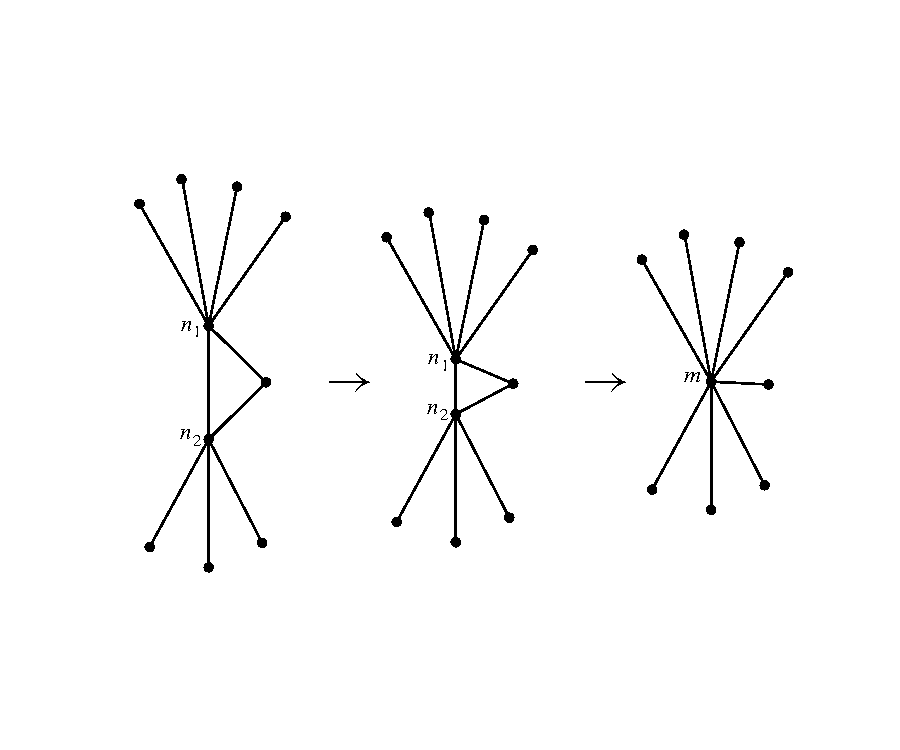
\includegraphics[height=4in]{vertex-merge-arrows}
\caption{Merging adjacent vertices $n_1$ and $n_2$ into new vertex, $m$.}
\label{fig:merged}
\end{figure}

For example, Figure~\ref{fig:5DL} illustrates why $C_3$ is a minor of
the graph in Figure~\ref{fig:5DL}(a).  In fact $C_3$ is a minor of a
connected graph~$G$ if and only if $G$ is not a tree.

\begin{figure}

\missinggraphic

\caption{One method by which the graph in~(a) can be reduced
  to~$C_3$~(f), thereby showing that $C_3$ is a minor of the graph.
  The steps are: merging the nodes incident to~$e_1$~(b),
  deleting~$v_1$ and all edges incident to it~(c), deleting $v_2$~(d),
deleting~$e_2$, and deleting $v_3$~(f).}

\label{fig:5DL}
\end{figure}

We will not prove Theorem~\ref{thm:kuratowski} here, nor will we prove
the following handy facts, which are obvious given the definition of a
planar drawing from Section~\ref{planar_graphs_sec}, and which can be
proved using the recursive definition of a planar embedding from
Section~\ref{sec:recdef_planar}.

\begin{corollary}\label{delete-vertex}
Deleting a vertex from a planar graph, along with all its incident
edges, leaves another planar graph.
\end{corollary}

\begin{theorem}\label{planar-subgraph}
  Any \index{planar subgraph}subgraph of a planar graph is planar.
\end{theorem}

\begin{theorem}\label{mergelem}
Merging two adjacent vertices of a planar graph leaves another planar
graph.
\end{theorem}

\subsection{Coloring Planar Graphs}

We've covered a lot of ground with planar graphs, but not nearly
enough to prove the famous 4-color theorem.  But we can get awfully
close.  Indeed, we have done almost enough work to prove that every
planar graph can be colored using only 5 colors.  We need only one
more lemma:
\begin{lemma}\label{lem:pg5}
Every planar graph has a vertex of degree at most five.
\end{lemma}

\begin{proof}
By contradiction.
If every vertex had degree at least~6, then the sum of the vertex
degrees is at least~$6v$, but since the sum of the vertex degrees
equals~$2e$, by the Handshake Lemma (Lemma~\ref{sumedges}), we have $e
\ge 3v$ contradicting the fact that $e \le 3v - 6 < 3v$ by
Theorem~\ref{e3v}.
\end{proof}

\begin{theorem}
Every planar graph is five-colorable.
\end{theorem}

\begin{proof}
The proof will be by strong induction on the number, $v$, of vertices, with
induction hypothesis:
\begin{quote}
Every planar graph with $v$ vertices is five-colorable.
\end{quote}

\inductioncase{Base cases} ($v \leq 5$): immediate.

\inductioncase{Inductive case}: Suppose $G$ is a planar graph with
$v+1$ vertices.  We will describe a five-coloring of $G$.

First, choose a vertex, $g$, of $G$ with degree at most 5;
Lemma~\ref{lem:pg5} guarantees there will be such a vertex.
\begin{description}

\item[Case 1:] ($\degr{g}<5$): Deleting $g$ from $G$ leaves a graph,
$H$, that is planar by Corollary~\ref{delete-vertex}, and, since $H$
has $v$ vertices, it is five-colorable by induction hypothesis.  Now
define a five coloring of $G$ as follows: use the five-coloring of $H$
for all the vertices besides $g$, and assign one of the five colors to
$g$ that is not the same as the color assigned to any of its
neighbors.  Since there are fewer than 5 neighbors, there will always
be such a color available for $g$.

\item[Case 2:] ($\degr{g}=5$): If the five neighbors of $g$ in $G$
  were all adjacent to each other, then these five vertices would form
  a nonplanar subgraph isomorphic to $K_5$, contradicting
  Theorem~\ref{planar-subgraph} (since $K_5$ is not planar).  So there
  must be two neighbors, $n_1$ and $n_2$, of $g$ that are not
  adjacent.  Now merge $n_1$ and $g$ into a new vertex,~$m$.  In this
  new graph, $n_2$ is adjacent to $m$, and the graph is planar by
  Theorem~\ref{mergelem}.  So we can then merge $m$ and $n_2$ into a
  another new vertex, $m'$, resulting in a new graph, $G'$, which by
  Theorem~\ref{mergelem} is also planar.  Since $G'$ has $v-1$
  vertices, it is five-colorable by the induction hypothesis.

\end{description}

Define a five coloring of $G$ as follows: use the five-coloring of $G'$
for all the vertices besides $g$, $n_1$ and $n_2$.  Next assign the color
of $m'$ in $G'$ to be the color of the neighbors $n_1$ and $n_2$.  Since
$n_1$ and $n_2$ are not adjacent in $G$, this defines a proper
five-coloring of $G$ except for vertex $g$.  But since these two neighbors
of $g$ have the same color, the neighbors of $g$ have been colored using
fewer than five colors altogether.  So complete the five-coloring of $G$ by
assigning one of the five colors to $g$ that is not the same as any of the
colors assigned to its neighbors.

\end{proof}

\subsection{Classifying \idx{Polyhedra}}

The \idx{Pythagoreans} had two great mathematical secrets, the
irrationality of $\sqrt{2}$ and a geometric construct that we're about
to rediscover!

A \term{polyhedron} is a convex, three-dimensional region bounded by a
finite number of polygonal faces.  If the faces are identical regular
polygons and an equal number of polygons meet at each corner, then the
polyhedron is \index{regular polyhedron}\term*{regular}.  Three
examples of regular polyhedra are shown in Figure~\ref{fig:polyhedra}: the
tetrahedron, the cube, and the octahedron.

\begin{figure}
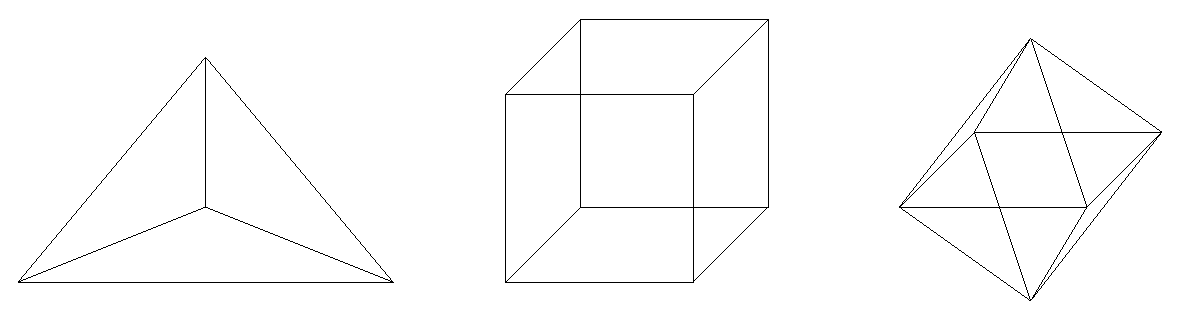
\includegraphics[height=1.25in]{polyhedra}
\missinggraphic[Add sublabels]
\caption{The tetrahedron~(a), cube~(b), and octahedron~(c).}
\label{fig:polyhedra}
\end{figure}

We can determine how many more regular polyhedra there are by thinking
about planarity.  Suppose we took \emph{any} polyhedron and placed a
sphere inside it.  Then we could project the polyhedron face
boundaries onto the sphere, which would give an image that was a
planar graph embedded on the sphere, with the images of the corners of
the polyhedron corresponding to vertices of the graph.  We've already
observed that embeddings on a sphere are the same as embeddings on the
plane, so Euler's formula for planar graphs can help guide our search
for regular polyhedra.

For example, planar embeddings of the three polyhedra in
Figure~\ref{fig:5DP} are shown in Figure~\ref{fig:5DQ}.

\begin{figure}
\setlength{\unitlength}{2000sp}%{3947sp}%
%
\begingroup\makeatletter\ifx\SetFigFont\undefined%
\gdef\SetFigFont#1#2#3#4#5{%
  \reset@font\fontsize{#1}{#2pt}%
  \fontfamily{#3}\fontseries{#4}\fontshape{#5}%
  \selectfont}%
\fi\endgroup%
\begin{picture}(9999,2124)(1489,-3073)
%\thinlines
{\color[rgb]{0,0,0}\put(8476,-3061){\line( 3, 4){1548}}
\put(9976,-961){\line( 3,-4){1548}}
\put(11476,-3061){\line(-1, 0){3000}}
}%
{\color[rgb]{0,0,0}\put(9526,-2011){\line( 1, 0){900}}
\put(10426,-2011){\line(-3,-5){450}}
\put(9976,-2761){\line(-3, 5){450}}
}%
{\color[rgb]{0,0,0}\put(8476,-3061){\line( 1, 1){1050}}
\put(9526,-2011){\line( 2, 5){424.138}}
}%
{\color[rgb]{0,0,0}\put(9976,-961){\line( 2,-5){424.138}}
\put(10426,-2011){\line( 1,-1){1050}}
}%
{\color[rgb]{0,0,0}\put(11476,-3061){\line(-5, 1){1500}}
\put(9976,-2761){\line(-5,-1){1500}}
}%
{\color[rgb]{0,0,0}\put(3001,-1261){\line(-5,-6){1500}}
\put(1501,-3061){\line( 1, 0){3000}}
\put(4501,-3061){\line(-5, 6){1500}}
\put(3001,-1261){\line( 0,-1){1200}}
\put(3001,-2461){\line(-5,-2){1500}}
}%
{\color[rgb]{0,0,0}\put(3001,-2461){\line( 5,-2){1500}}
}%
{\color[rgb]{0,0,0}\put(5401,-3061){\framebox(2100,2100){}}
}%
{\color[rgb]{0,0,0}\put(6001,-2461){\framebox(900,900){}}
}%
{\color[rgb]{0,0,0}\put(5401,-961){\line( 1,-1){600}}
}%
{\color[rgb]{0,0,0}\put(5401,-3061){\line( 1, 1){600}}
}%
{\color[rgb]{0,0,0}\put(7501,-3061){\line(-1, 1){600}}
}%
{\color[rgb]{0,0,0}\put(7501,-961){\line(-1,-1){600}}
}%
\end{picture}%

\caption{Planar embeddings of the tetrahedron~(a), cube~(b, and
  octahedron~(c).}
\label{fig:5DQ}
\end{figure}

Let $m$ be the number of faces that meet at each corner of a
polyhedron, and let $n$ be the number of edges on each face.  In the
corresponding planar graph, there are $m$ edges incident to each of
the $v$ vertices.  By the Handshake Lemma~\ref{sumedges}, we
know:
%
\[
m v = 2 e.
\]
%
Also, each face is bounded by $n$ edges.  Since each edge is on the
boundary of two faces, we have:
%
\[
n f = 2 e
\]
%
Solving for $v$ and $f$ in these equations and then substituting into
\idx{Euler's formula} gives:
\[
\frac{2e}{m} - e + \frac{2e}{n} = 2
\]
which simplifies to
\begin{equation}\label{1m1n}
\frac{1}{m} + \frac{1}{n} = \frac{1}{e} + \frac{1}{2}
\end{equation}
%
Equation~\ref{1m1n} places strong restrictions on the structure of a
polyhedron.  Every nondegenerate polygon has at least 3 sides, so $n
\geq 3$.  And at least 3 polygons must meet to form a corner, so $m
\geq 3$.  On the other hand, if either $n$ or $m$ were 6 or more, then
the left side of the equation could be at most $1/3 + 1/6 = 1/2$,
which is less than the right side.  Checking the finitely-many cases
that remain turns up only five solutions, as shown in
Figure~\ref{fig:5DR}.  For each valid combination of $n$ and $m$, we
can compute the associated number of vertices $v$, edges $e$, and
faces $f$.  And polyhedra with these properties do actually exist.
The largest polyhedron, the dodecahedron, was the other great
mathematical secret of the Pythagorean sect.

\begin{figure}

\[
\begin{array}{cc|ccc|l}
n & m & v  & e  &  f & \text{polyhedron} \\ \hline
3 & 3 & 4  & 6  &  4 & \text{tetrahedron} \\
4 & 3 & 8  & 12 &  6 & \text{cube} \\
3 & 4 & 6  & 12 &  8 & \text{octahedron} \\
3 & 5 & 12 & 30 & 20 & \text{icosahedron} \\
5 & 3 & 20 & 30 & 12 & \text{dodecahedron}
\end{array}
\]

\caption{The only possible regular polyhedra.}

\label{fig:5DR}

\end{figure}

The 5 polyhedra in Figure~\ref{fig:5DR} are the only possible regular
polyhedra.  So if you want to put more than 20 geocentric satellites
in orbit so that they \emph{uniformly} blanket the globe---tough luck!

\section{Problems}

%% Planar Graphs Problems %%%%%%%%%%%%%%%%%%%%%%%%%%%%%%%%%%%%%%%%%%%%%%%%%%%%%
\begin{problems}

\examproblems
\pinput{MQ_planar_isomorphism}

\classproblems
\pinput{CP_planar_embedding_isomorphism}
\pinput{CP_K33_not_planar}
\pinput{CP_planar_structural_induction}

\homeworkproblems
\pinput{PS_triangle_free_planar_graphs}
\pinput{PS_planar_graph_construction_order}

%\pinput{CP0506_}
\end{problems}

%% Conclusion %%%%%%%%%%%%%%%%%%%%%%%%%%%%%%%%%%%%%%%%%%%%%%%%%%%%%%%%%%%%%%%%%
%\TBA{Add conclusion here...}

\endinput


%% Conclusion %%%%%%%%%%%%%%%%%%%%%%%%%%%%%%%%%%%%%%%%%%%%%%%%%%%%%%%%%%%%%%%%%
%\TBA{Add conclusion here...}

\endinput
